\documentclass[aspectratio=169,10pt]{beamer}
\usetheme{Madrid}
\usepackage[T1]{fontenc}

\usepackage{fancybox,graphicx,hyperref,url}
\usepackage{tikz}
\usetikzlibrary{fit}
\usetikzlibrary{shadings}
\usetikzlibrary{shapes.arrows,shadows.blur}
\usetikzlibrary{shapes,arrows}
\usetikzlibrary{positioning}
\usetikzlibrary{calc, chains, decorations.pathmorphing}
\usetikzlibrary{shapes,arrows,backgrounds}
\usetikzlibrary{positioning,fit,shapes.geometric,shapes}
\usepackage{physics}
\usepackage{amsmath}
\usepackage{tikz}
\usepackage{mathdots}
\usepackage{yhmath}
\usepackage{cancel}
\usepackage{color}
\usepackage{siunitx}
\usepackage{array}
\usepackage{multirow}
\usepackage{amssymb}
\usepackage{gensymb}
\usepackage{tabularx}
\usepackage{extarrows}
\usepackage{booktabs}
\usetikzlibrary{fadings}
\usetikzlibrary{patterns}
\usetikzlibrary{shadows.blur}
\usetikzlibrary{shapes}

\usepackage{booktabs}
\usepackage{enumitem}

\usepackage{listings}
\usepackage{lstautogobble}
% Stolen from https://raw.githubusercontent.com/lammich/isabelle_llvm/2022/papers/ITP2022/lstisabelle.tex
% Not really meant for highlighting isabelle source, but for easily writing latex that looks like
% isabelle
%
% keyword level 1 - isabelle outer syntax
% keyword level 2 - isabelle inner syntax programming constructs (if, let, etc)
% keyword level 3 - standard constants (length, mod, etc)
% keyword level 4 - isabelle proof methods


% \newcommand{\lsem}{\ensuremath{\mathopen{[\![}}}
% \newcommand{\rsem}{\ensuremath{\mathclose{]\!]}}}

\lstdefinelanguage{isabelle}{
  morekeywords={theorem,theorems,corollary,lemma,lemmas,locale,sublocale,global_interpretation,begin,end,fixes,assumes,shows,and,class,
    constrains , definition, abbreviation, defines, where, done,unfolding, primrec, primcorec, inductive, coinductive, corecursive, corec, friend_of_corec, partial_function, fun, function, using, by, for, uses, file,
    schematic_lemma, concrete_definition, prepare_code_thms, export_code, datatype, codatatype, type_synonym, typedef, value,
    proof, next, qed, show, have, hence, thus, interpretation, fix, context, sepref_definition,is,export_llvm
 } ,
  morekeywords=[2]{rec, return, bind, foreach, if, then, else, do, let, in, res, spec, fail, assert, assume, while, case, of,
    check,with_split,npar,nseq},
  morekeywords=[3]{LNil, LCons, ltl, lhd, lnull, lmap, lset, Cons, None, Some, the, lfind, Logic, fold, produce, produce_inner, count_op, while_option, LEAST, ^^, snd, fst, produce_inner_aux, hd, tl,
    produce_1', produce_1, produce_induct, @, fproduce, comp_op, produce_comp_op_correctness, produce_1_comp_op_None_fproduce, skip_op, cong,
    ldropn, produce_1_comp_op_None_fproduce, WM, wmk, tmp, data, DT, insert, monotone, LConsR, LConsL, productive, EnvWM, EnvDT, LFinite, monotone_cong, monotone_cong_prepend, vimage, Suc,
    length, llength, set_t, tmps, drop, nth, coinduction, lfinite, llist_of, batch_op, filter, lfilter, incr_op, remdups, rev, map, List, map_filter, mset, case_event, Map, empty, lfilter, case_event, list_of,
    data_at, data_at_from_list, lcoll, coll, mono_prod, set, batch_coll_sound, get_Data, enat, ts, ws, batch_ts, lnth, batch_ts_sound, undefined, LNil_lprefix, LCons_lprefix, In_llist, Next_llist, in_llist,
    EZero, ESucc, ltake, pf_prod, pf_stop, pf_step, concat, snd, ltake_DT, the_enat, acc_batches, incr_batch_op, maxchain, paths, lpaths, incr_lcoll, incr_coll, sum, map_op, incr_hist_op,
    join_op, flatten_op, join_list, union_op, Inl, Inr, apply, Inl_leq, Inr_leq, incr_hist_op', eq_op, eq_op_lifted, WM, rel_prod, EQ, less_eq_sum, Pow, prefix, exit,
    monotone_cong_base, productive_cong, productive_cong_base, productive_cong_prepend, wms, lapp, lconcat, lprefix, lfilter, lshift, @@, lSup, THE},
%   morekeywords=[4]{simp,auto,intro,elim,rprems,refine_mono,refine_rcg},
  sensitive=True,
  morecomment=[s]{(\*}{\*)},
  moredelim=*[is][\ttfamily]{**}{**},
}


\DeclareTextCommand{\shortunderscore}{T1}{%
  \leavevmode \kern.06em\vbox{\hrule width.4em}}

\renewcommand{\textunderscore}{\shortunderscore}

\lstset{
    language=isabelle,
    upquote=true,
    mathescape=true,
    escapeinside={--"}{"},
    basicstyle={\itshape},
    keywordstyle=\rm\bfseries,
    keywordstyle=[2]\rm\tt,
    keywordstyle=[3]\rm\sffamily,
    keywordstyle=[4]\rm,
    keywordstyle=[5]\rm\bfseries,
    showstringspaces=false,
    keepspaces=true,
    columns=[c]fullflexible}
\lstset{literate=
  {"}{}0
%  {'}{{${}^\prime\!$}}1
  %{''}{{${}^\prime$}}1
  {'}{{${}^\prime$}}1
  {~:}{{$\notin$}}1
  {\%}{{$\lambda$}}1
  {\\\%}{{$\lambda$}}1
  {\\\$}{{$\mathbin{\,\$\,}$}}1
  {&}{{$\wedge$}}1
  {?}{{$\exists$}}1
%  {!}{{$\forall$}}1 clashes with nth xs!i
  {->}{{$\rightarrow$}}1
  {<-}{{$\leftarrow$}}1
%   {<.}{{$\langle$}}1
%   {.>}{{$\rangle$}}1
  {<=}{{$\le$}}1
  {>=}{{$\ge$}}1
  {<->}{{$\leftrightarrow$}}1
  {-->}{{$\longrightarrow$}}2
  {-->>}{{$\boldsymbol{\longrightarrow}$}}5
  {<-->}{{$\longleftrightarrow$}}1
  {=>}{{$\Rightarrow$}}1
  {==}{{$\equiv$}}2
  {==>}{{$\implies$}}2
  {<=>}{{$\Leftrightarrow$}}1
  {~=}{{$\ne$}}1
  {|}{{$\mid$}}1
  % {-`}{$vimage$}1
  {|`}{{$\restriction$}}1
  {!!}{{$\bigwedge$}}1
  {(}{{$($}}1
  {)}{{$)$}}1
  {\{}{{$\{$}}1
  {\}}{{$\}$}}1
  {[}{{$[$}}1
  {]}{{$]$}}1
  {[|}{{$\llbracket$}}1
  {|]}{{$\rrbracket$}}1
  {\\<lbrakk>}{{$\lsem$}}1
  {\\<rbrakk>}{{$\rsem$}}1
  {|-}{{$\vdash$}}1
  {|=}{{$\models$}}1
  {|->}{{$\mapsto$}}1
  {|_|}{{$\bigsqcup$}}1
  {...}{{$\dots$}}1
  {\\x}{{$\times$}}1
  {_0}{{${}_0$}}1
  {_1}{{${}_1$}}1
  {_2}{{${}_2$}}1
  {_3}{{${}_3$}}1
  {_4}{{${}_4$}}1
  {_5}{{${}_5$}}1
  {_6}{{${}_6$}}1
  {_7}{{${}_7$}}1
  {_8}{{${}_8$}}1
  {_9}{{${}_9$}}1
  {_L}{{${}_L$}}1
  {\\_n}{{${}_n$}}1
  {\\_i}{{${}_i$}}1
  {\\_j}{{${}_j$}}1
  {\\_x}{{${}_x$}}1
  {\\_y}{{${}_y$}}1
  {\\impl}{{${}_\dagger$}}1
  {^*}{{$^*$}}1
  {^k}{{$^k$}}1
  {^d}{{$^d$}}1
  {\\<^sup>*}{{$^*$}}1
  {\\<^sub>*}{{$_*$}}1
  {\\<^sub>A}{{$_A$}}1
  {\\<^sub>r}{{$_r$}}1
  {\\<^sub>a}{{$_a$}}1
  {:_i}{{$:_i$}}1
  {\\<A>}{{$\mathcal{A}$}}1
  {\\<O>}{{\sf o}}1
  {\\<Phi>}{{$\Phi$}}1
  {\\<phi>}{{$\phi$}}1
  {\\<Psi>}{{$\Psi$}}1
  {\\<sigma>}{{$\sigma$}}1
  {\\<Sigma>}{{$\Sigma$}}1
  {\\<cdot>}{{$\cdot$}}1
  {\\<in>}{{$\in$}}1
  {\\<le>}{{$\le$}}1
  {\\<noteq>}{{$\ne$}}1
  {\\<lambda>}{{$\lambda$}}1
  {\\<longrightarrow>}{{$\longrightarrow$}}1
  {\\<longleftrightarrow>}{{$\longleftrightarrow$}}1
  {\\<Rightarrow>}{{$\Rightarrow$}}1
  {\\<Longrightarrow>}{{$\Longrightarrow$}}1
  {\\<rightarrow>}{{$\rightarrow$}}1
  {\\<leftarrow>}{{$\leftarrow$}}1
  {\\<mapsto>}{{$\mapsto$}}1
  {\\<equiv>}{{$\equiv$}}1
  {\\<and>}{{$\wedge$}}1
  {\\<or>}{{$\vee$}}1
  {\\<And>}{{$\bigwedge$}}1
  {\\<Up>}{{$\Uparrow$}}1
  {\\<Down>}{{$\Downarrow$}}1
  {\\<Union>}{{$\bigcup$}}1
  {\\<up>}{{$\uparrow$}}1
  {\\<down>}{{$\downarrow$}}1
  {\\<times>}{{$\times$}}1
  {\\<forall>}{{$\forall$}}1
  {\\<exists>}{{$\exists$}}1
  {\\<nexists>}{{$\nexists$}}1
  {\\<union>}{{$\cup$}}1
  {\\<inter>}{{$\cap$}}1
  {\\in}{$\in$}1
  {\\union}{{$\cup$}}1
  {\\inter}{{$\cap$}}1
  {\\<subset>}{{$\subset$}}1
  {\\<subseteq>}{{$\subseteq$}}1
  {\\<supset>}{{$\supset$}}1
  {\\<supseteq>}{{$\supseteq$}}1
  {\\<alpha>}{{$\alpha$}}1
  {\\<beta>}{{$\beta$}}1
  {\\<gamma>}{{$\gamma$}}1
  {\\alpha}{{$\alpha$}}1
  {\\beta}{{$\beta$}}1
  {\\gamma}{{$\gamma$}}1
  {\\rho}{{$\rho$}}1
  {\\<rho>}{{$\rho$}}1
  {\\<Gamma>}{{$\Gamma$}}1
  {\\<langle>}{{$\langle$}}1
  {\\<rangle>}{{$\rangle$}}1
  {\\<not>}{{$\neg$}}1
  {\\<box>}{{$\oblong$}}1
  {\\<bot>}{{$\bot$}}1
  {\\<top>}{{$\top$}}1
  {\\<notin>}{{$\notin$}}1
  {\\<guillemotright>}{{$\gg$}}1
  {\\approx}{$\approx$}1
  {\\<approx>}{$\approx$}1
  {\\and}{$\wedge$}1
  {\\or}{$\vee$}1
  {\\mu}{$\mu$}1
  {\\Phi}{{$\Phi$}}1
  {\\Psi}{{$\Psi$}}1
  {\\le}{{$\le$}}1
  {\\Up}{{$\Uparrow$}}1
  {\\Down}{{$\Down$}}1
  {>>}{{$\gg$}}1
  {>>=}{{${\gg}{=}$}}1
  {<*lex*>}{{$\times_{\sf lex}$}}1
  {\\<open>}{{\rm\guilsinglleft}}1
  {\\<close>}{{\rm\guilsinglright}}1
  {\\<box>}{{$\square$}}1
  {\\<proof>}{{\color{darkgray}$\langle\text{proof}\rangle$}}7
}

\newcommand*{\rightcomment}[1]{\hfill\color{darkgray} --- #1}%

% \newcommand{\is}{\lstinline[language=isabelle,basicstyle=\normalsize\ttfamily\slshape]}
\newcommand{\is}{\lstinline[language=isabelle]}%, breaklines=true]}
\newcommand{\cs}{\lstinline[language=C++]}
\newcommand{\q}[1]{\mbox{\guilsinglleft{#1}\hspace{-.0pt}\guilsinglright}}
% \newcommand{\isai}[1]{\q{\lstinline[language=isabelle,basicstyle=\normalsize\ttfamily\slshape]{#1}}}
% \cMakeRobust

\usepackage[listings,skins,breakable,xparse]{tcolorbox}
\tcbuselibrary{theorems}
\tcbset{highlight math/.append style={boxrule=0pt,
                                      frame hidden,
                                      colback=yellow!40!white,
                                      sharp corners}}

\usepackage{xpatch}
\usepackage{xcolor}
\usepackage{realboxes}

\pgfdeclarefunctionalshading{Hermite-Gaussian modes}{\pgfpoint{-25bp}{-25bp}}{\pgfpoint{25bp}{25bp}}{}{
    10 atan sin 1000 mul cos 1 add
    exch
    10 atan sin 1000 mul cos 1 add
    mul 4 div
    dup dup
}

\makeatletter
\xpretocmd\lstinline{\Colorbox{yellow!10!white}\bgroup\appto\lst@DeInit{\egroup}}{}{}
\makeatother

\definecolor{my_red}{RGB}{128, 0, 0}

\lstset{captionpos=b}
\lstset{numberbychapter=false}
\lstset{autogobble}
% \lstset{breaklines=true}

\usepackage{subcaption}

\setbeamercovered{transparent}

\setlistdepth{9}
\setlist[itemize,1]{label=$\bullet$}
\setlist[itemize,2]{label=$\bullet$}
\setlist[itemize,3]{label=$\bullet$}
\setlist[itemize,4]{label=$\bullet$}
\setlist[itemize,5]{label=$\bullet$}
\setlist[itemize,6]{label=$\bullet$}
\setlist[itemize,7]{label=$\bullet$}
\setlist[itemize,8]{label=$\bullet$}
\setlist[itemize,9]{label=$\bullet$}
\renewlist{itemize}{itemize}{9}

\setlist[enumerate,1]{label=$\arabic*.$}
\setlist[enumerate,2]{label=$\alph*.$}
\setlist[enumerate,3]{label=$\roman*.$}
\setlist[enumerate,4]{label=$\arabic*.$}
\setlist[enumerate,5]{label=$\alpha*$}
\setlist[enumerate,6]{label=$\roman*.$}
\setlist[enumerate,7]{label=$\arabic*.$}
\setlist[enumerate,8]{label=$\alph*.$}
\setlist[enumerate,9]{label=$\roman*.$}
\renewlist{enumerate}{enumerate}{9}

\AtBeginSection[]{
  \begin{frame}[noframenumbering]
    \vfill
    \centering
    \begin{beamercolorbox}[sep=8pt,center,shadow=true,rounded=true]{title}
      \usebeamerfont{title}\insertsectionhead\par%
    \end{beamercolorbox}
    \vfill
  \end{frame}
}

\title[Efficient and Verified Non-Terminating Programs with Isabelle-LLVM]{Efficient and Verified Non-Terminating Programs with Isabelle-LLVM}

\author[Rafael Castro]{
  Rafael Castro G. Silva\\\medskip
  {\small \url{rasi@di.ku.dk}}}

\date{23/11/2023}

\institute[UCPH]{
  Department of Computer Science \\
  University of Copenhagen}

\begin{document}
\setbeamercovered{invisible}
% \setbeamercovered{dynamic}

\begin{frame}
  \titlepage

\end{frame}

\section{Introduction}

\begin{frame}[fragile]
  \frametitle{Context}
  \begin{itemize}
          \pause
    \item Distributed Systems
          \begin{itemize}
            \item Stream processing frameworks
                  \begin{itemize}
                    \item Dataflow models
                          \begin{itemize}
                            \item Time-Aware Computations
                          \end{itemize}
                  \end{itemize}
          \end{itemize}
          \pause
    \item Formal Methods
          \begin{itemize}
            \item Verification using proof assistants
                  \begin{itemize}
                    \item Isabelle proofs
                          \begin{itemize}
                            \item Verified + executable + efficient code
                          \end{itemize}
                  \end{itemize}
          \end{itemize}
    \item Formalization of Time-Aware Stream Processing
  \end{itemize}
\end{frame}


\begin{frame}[fragile]
  \frametitle{Stream Processing}
  \begin{itemize}
    \item Stream Processing: Abstraction for processing data when the input is not completely presented in the begging of the computation
          \pause
    \item Dataflow Model:
          \begin{itemize}
            \item Directed graph of interconnected operators that perform event-wise transformations
            \item E.g.: Apache Flink, Apache Samza, Apache Spark, Google Cloud Dataflow, and Timely Dataflow
                  \vspace*{-1ex}
                  \begin{overlayarea}{\textwidth}{.15\textheight}
                    \centering
                    \begin{figure}
                      \centering
                      \only<2->{
\includegraphics[scale=0.15]{all.png}}
                    \end{figure}
                  \end{overlayarea}
                  \vspace*{-1ex}
            \item Highly Parallel
                  \vspace*{-1ex}
                  \begin{figure}
                    \begin{subfigure}{0.45\linewidth}
                      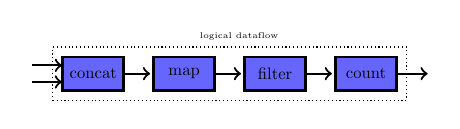
\begin{tikzpicture}[node distance = 0.6cm, scale=0.6, transform shape]]
                        \tikzstyle{operator} = [rectangle, draw, fill=blue!60, text width=3.0em, text centered, minimum height=20pt, line width=1pt]

                        \node [operator] at (0,0)  (concat) {concat};
                        \node [operator, right = of concat] (map) {map};
                        \node [operator, right = of map] (filter) {filter};
                        \node [operator, right = of filter] (count) {count};

                        \draw[<-,thick,shorten >=1pt] ([yshift=5pt]concat.west)  -- node[above]{} ++(-2em,0em);
                        \draw[<-,thick,shorten >=1pt] ([yshift=-5pt]concat.west)  -- node[above]{} ++(-2em,0em);
                        \draw [thick,->,shorten >=1pt] (concat) -- (map);
                        \draw [thick,->,shorten >=1pt] (map) -- (filter);
                        \draw [thick,->,shorten >=1pt] (filter) -- (count);
                        \draw[->,thick,shorten >=1pt] (count.east)  -- node[above]{} ++(2em,0em);

                        \node[draw,densely dotted, label={[xshift=2mm]above:{\tiny logical dataflow}},fit=(concat) (map) (filter) (count)] {};

                      \end{tikzpicture}
                    \end{subfigure}
                    \begin{subfigure}{0.45\linewidth}
                      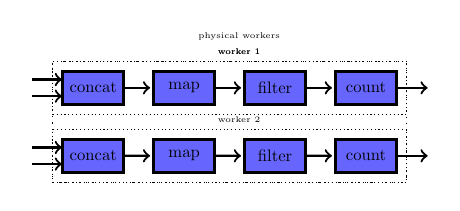
\begin{tikzpicture}[node distance = 0.6cm,auto, scale=0.6, transform shape]]
                        \tikzstyle{operator} = [rectangle, draw, fill=blue!60, text width=3.0em, text centered, minimum height=20pt, line width=1pt]

                        \node [operator] at (0,0)  (concat) {concat};
                        \node [operator, right = of concat] (map) {map};
                        \node [operator, right = of map] (filter) {filter};
                        \node [operator, right = of filter] (count) {count};

                        \draw[<-,thick,shorten >=1pt] ([yshift=5pt]concat.west)  -- node[above]{} ++(-2em,0em);
                        \draw[<-,thick,shorten >=1pt] ([yshift=-5pt]concat.west)  -- node[above]{} ++(-2em,0em);
                        \draw [thick,->,shorten >=1pt] (concat) -- (map);
                        \draw [thick,->,shorten >=1pt] (map) -- (filter);
                        \draw [thick,->,shorten >=1pt] (filter) -- (count);
                        \draw[->,thick,shorten >=1pt] (count.east)  -- node[above]{} ++(2em,0em);

                        \node[draw,densely dotted, label={[xshift=2mm]above:{\tiny worker 1}},fit=(concat) (map) (filter) (count)] {};

                        \node [operator, below=0.7cm of concat]  (concat') {concat};
                        \node [operator, right = of concat'] (map') {map};
                        \node [operator, right = of map'] (filter') {filter};
                        \node [operator, right = of filter'] (count') {count};

                        \draw[<-,thick,shorten >=1pt] ([yshift=5pt]concat'.west)  -- node[above]{} ++(-2em,0em);
                        \draw[<-,thick,shorten >=1pt] ([yshift=-5pt]concat'.west)  -- node[above]{} ++(-2em,0em);
                        \draw [thick,->,shorten >=1pt] (concat') -- (map');
                        \draw [thick,->,shorten >=1pt] (map') -- (filter');
                        \draw [thick,->,shorten >=1pt] (filter') -- (count');
                        \draw[->,thick,shorten >=1pt] (count'.east)  -- node[above]{} ++(2em,0em);

                        \node[draw,densely dotted, label={[xshift=2mm]above:{\tiny worker 1}},fit=(concat) (map) (filter) (count)] {};
                        \node[draw,densely dotted, label={[xshift=2mm]above:{\tiny worker 2}},fit=(concat') (map') (filter') (count')] {};
                        \node[draw,dotted, label={[xshift=2mm, yshift=0.3cm]above:{\tiny physical workers}},fit=(concat') (concat) (map') (map) (filter) (filter') (count) (count')] {};
                      \end{tikzpicture}
                    \end{subfigure}
                  \end{figure}
          \end{itemize}
                  \vspace*{-1ex}
  \end{itemize}
\end{frame}

\begin{frame}[fragile]
  \frametitle{Time-Aware Stream Processing (part 1)}
  \begin{itemize}
    \item Time-Aware Computations:
          \begin{itemize}
            \item Timestamps: Metadata associating the data with some data collection
                  \begin{itemize}
                    \item An unix timestamp
                    \item Version of the data
                    \item Logical grouping
                  \end{itemize}
            \item Watermarks: Metadata indicating the completion of a data collection
                  \begin{itemize}
                    \item e.g.: A watermark 5 says that there is no data associated with timestamp 5 or bellow arriving
                    \item Are increasingly monotonic (they don't go backwards in time)
                  \end{itemize}
            \item e.g.:
  \begin{figure}[!t]
      \raggedright
        \begin{tikzpicture}[scale=0.8, every node/.style={scale=0.8},background rectangle/.style={fill=yellow!10!white},show background rectangle]
          \tikzset{tape/.style={minimum size=.6cm, draw}}
          \begin{scope}[start chain=0 going right, node distance=0mm]
            \foreach \x [count=\i] in {\is{DT t_4 **d**},\is{DT t_0 **a**},\is{DT t_1 **c**},\is{WM t_1},\is{DT t_2 **b**}, \is{WM t_2},\is{DT t_5 **c**},\is{DT t_3 **a**},\is{DT t_5 **a**},\is{WM t_5}} {
                \node [on chain=0, tape] (n\i) {\x};
            }
            \node [right=.05cm of n10] {$\cdots$};
          \end{scope}
        \end{tikzpicture}
    \end{figure}
          \end{itemize}
  \end{itemize}
\end{frame}

% \draw (55,142) node [anchor=north west][inner sep=0.75pt]   [align=left] {$\lambda$ e. case e of\\DT t d => insert (t, d) buf\\WM wm =>\\ \ if $\exists$ t $\in$ (map fst buf). \ t \ $\le$ wm\\ \ then\\ \ \ \ out <- filter ($\lambda$ (t, \_) . t $\le$ wm) buf\\ \ \ \ \ ts <- remdups (map fst out)\\ \ \ \ \ buf <- filter ($\lambda$ (t, \_) . t > wm) buf\\ \ \ \ \ H <- H + (mset (map snd out))\\ \ \ \ \ push (map ($\lambda$ t . DT t (H + (mset (map snd (filter ($\lambda$ (t', \_) . t' $\le$ t) out))))) ts) @ [WM wm]\\ \ else\\ \ \ \ \ push \ [WM wm]};

% https://www.mathcha.io/editor
\begin{frame}[fragile]
  \frametitle{Example of Time-Aware Stream Processing}


\tikzset{every picture/.style={line width=0.75pt}} %set default line width to 0.75pt

\resizebox{0.9\textwidth}{0.8\textheight}{%
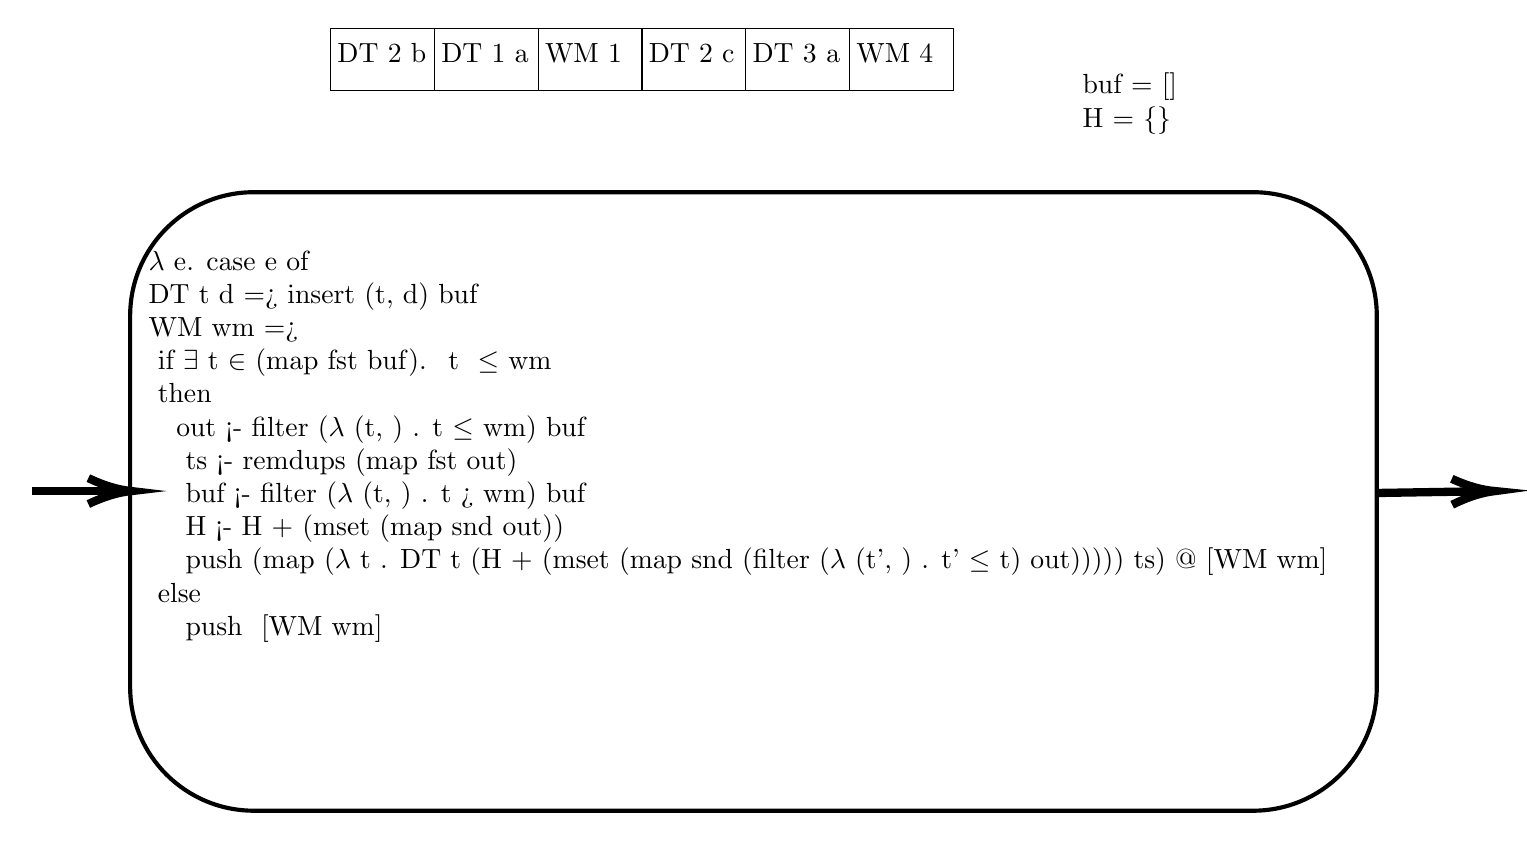
\begin{tikzpicture}[x=0.75pt,y=0.75pt,yscale=-1,xscale=1]
%uncomment if require: \path (0,489); %set diagram left start at 0, and has height of 489

%Rounded Rect [id:dp2828185464138784]
\draw  [line width=1.5]  (47.37,174.6) .. controls (47.37,141.68) and (74.05,115) .. (106.97,115) -- (588.4,115) .. controls (621.32,115) and (648,141.68) .. (648,174.6) -- (648,353.4) .. controls (648,386.32) and (621.32,413) .. (588.4,413) -- (106.97,413) .. controls (74.05,413) and (47.37,386.32) .. (47.37,353.4) -- cycle ;
%Shape: Rectangle [id:dp8322547950272192]
\draw   (144,36) -- (194,36) -- (194,66) -- (144,66) -- cycle ;
%Shape: Rectangle [id:dp16185128837259355]
\draw   (194,36) -- (244,36) -- (244,66) -- (194,66) -- cycle ;
%Shape: Rectangle [id:dp07527633485084895]
\draw   (244,36) -- (294,36) -- (294,66) -- (244,66) -- cycle ;
%Shape: Rectangle [id:dp6518760155585928]
\draw   (294,36) -- (344,36) -- (344,66) -- (294,66) -- cycle ;
%Shape: Rectangle [id:dp8004967249958459]
\draw   (344,36) -- (394,36) -- (394,66) -- (344,66) -- cycle ;
%Shape: Rectangle [id:dp6426296003908789]
\draw   (394,36) -- (444,36) -- (444,66) -- (394,66) -- cycle ;
%Straight Lines [id:da3914639201104144]
\draw [line width=3]    (0,259) -- (43,259) ;
\draw [shift={(48,259)}, rotate = 180] [color={rgb, 255:red, 0; green, 0; blue, 0 }  ][line width=3]    (20.77,-6.25) .. controls (13.2,-2.65) and (6.28,-0.57) .. (0,0) .. controls (6.28,0.57) and (13.2,2.66) .. (20.77,6.25)   ;
%Straight Lines [id:da5752451790936068]
\draw [line width=3]    (648,259.92) -- (700,259.08) ;
\draw [shift={(705,259)}, rotate = 179.08] [color={rgb, 255:red, 0; green, 0; blue, 0 }  ][line width=3]    (20.77,-6.25) .. controls (13.2,-2.65) and (6.28,-0.57) .. (0,0) .. controls (6.28,0.57) and (13.2,2.66) .. (20.77,6.25)   ;

% Text Node
\draw (146,42) node [anchor=north west][inner sep=0.75pt]   [align=left] {DT 2 b};
% Text Node
\draw (196,42) node [anchor=north west][inner sep=0.75pt]   [align=left] {DT 1 a};
% Text Node
\draw (246,42) node [anchor=north west][inner sep=0.75pt]   [align=left] {WM 1 };
% Text Node
\draw (296,42) node [anchor=north west][inner sep=0.75pt]   [align=left] {DT 2 c};
% Text Node
\draw (346,42) node [anchor=north west][inner sep=0.75pt]   [align=left] {DT 3 a};
% Text Node
\draw (396,42) node [anchor=north west][inner sep=0.75pt]   [align=left] {WM 4};
% Text Node
\draw (55,142) node [anchor=north west][inner sep=0.75pt]   [align=left] {$\lambda$ e. case e of\\DT t d => insert (t, d) buf\\WM wm =>\\ \ if $\exists$ t $\in$ (map fst buf). \ t \ $\le$ wm\\ \ then\\ \ \ \ out <- filter ($\lambda$ (t, \_) . t $\le$ wm) buf\\ \ \ \ \ ts <- remdups (map fst out)\\ \ \ \ \ buf <- filter ($\lambda$ (t, \_) . t > wm) buf\\ \ \ \ \ H <- H + (mset (map snd out))\\ \ \ \ \ push (map ($\lambda$ t . DT t (H + (mset (map snd (filter ($\lambda$ (t', \_) . t' $\le$ t) out))))) ts) @ [WM wm]\\ \ else\\ \ \ \ \ push \ [WM wm]};
% Text Node
\draw (505,56.33) node [anchor=north west][inner sep=0.75pt]   [align=left] {buf = []\\H = \{\}};
\end{tikzpicture}
}

\end{frame}


\begin{frame}[fragile, noframenumbering]
  \frametitle{Example of Time-Aware Stream Processing}
\tikzset{every picture/.style={line width=0.75pt}} %set default line width to 0.75pt

  \resizebox{0.9\textwidth}{0.8\textheight}{%

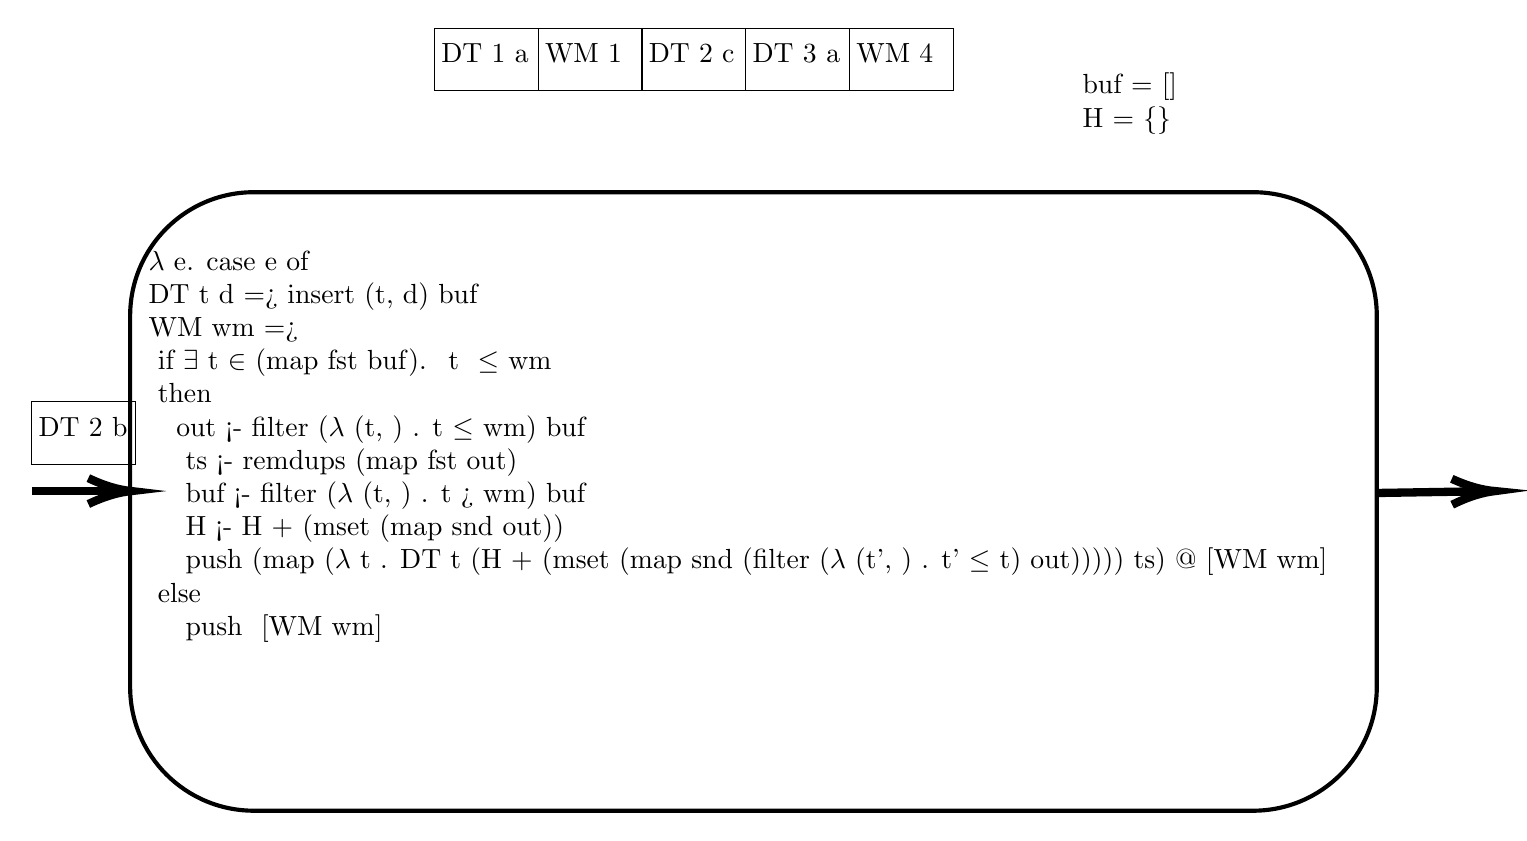
\begin{tikzpicture}[x=0.75pt,y=0.75pt,yscale=-1,xscale=1]
%uncomment if require: \path (0,489); %set diagram left start at 0, and has height of 489

%Rounded Rect [id:dp2828185464138784]
\draw  [line width=1.5]  (47.37,174.6) .. controls (47.37,141.68) and (74.05,115) .. (106.97,115) -- (588.4,115) .. controls (621.32,115) and (648,141.68) .. (648,174.6) -- (648,353.4) .. controls (648,386.32) and (621.32,413) .. (588.4,413) -- (106.97,413) .. controls (74.05,413) and (47.37,386.32) .. (47.37,353.4) -- cycle ;
%Shape: Rectangle [id:dp8322547950272192]
\draw   (0,216) -- (50,216) -- (50,246) -- (0,246) -- cycle ;
%Shape: Rectangle [id:dp16185128837259355]
\draw   (194,36) -- (244,36) -- (244,66) -- (194,66) -- cycle ;
%Shape: Rectangle [id:dp07527633485084895]
\draw   (244,36) -- (294,36) -- (294,66) -- (244,66) -- cycle ;
%Shape: Rectangle [id:dp6518760155585928]
\draw   (294,36) -- (344,36) -- (344,66) -- (294,66) -- cycle ;
%Shape: Rectangle [id:dp8004967249958459]
\draw   (344,36) -- (394,36) -- (394,66) -- (344,66) -- cycle ;
%Shape: Rectangle [id:dp6426296003908789]
\draw   (394,36) -- (444,36) -- (444,66) -- (394,66) -- cycle ;
%Straight Lines [id:da3914639201104144]
\draw [line width=3]    (0,259) -- (43,259) ;
\draw [shift={(48,259)}, rotate = 180] [color={rgb, 255:red, 0; green, 0; blue, 0 }  ][line width=3]    (20.77,-6.25) .. controls (13.2,-2.65) and (6.28,-0.57) .. (0,0) .. controls (6.28,0.57) and (13.2,2.66) .. (20.77,6.25)   ;
%Straight Lines [id:da5752451790936068]
\draw [line width=3]    (648,259.92) -- (700,259.08) ;
\draw [shift={(705,259)}, rotate = 179.08] [color={rgb, 255:red, 0; green, 0; blue, 0 }  ][line width=3]    (20.77,-6.25) .. controls (13.2,-2.65) and (6.28,-0.57) .. (0,0) .. controls (6.28,0.57) and (13.2,2.66) .. (20.77,6.25)   ;

% Text Node
\draw (2,222) node [anchor=north west][inner sep=0.75pt]   [align=left] {DT 2 b};
% Text Node
\draw (196,42) node [anchor=north west][inner sep=0.75pt]   [align=left] {DT 1 a};
% Text Node
\draw (246,42) node [anchor=north west][inner sep=0.75pt]   [align=left] {WM 1 };
% Text Node
\draw (296,42) node [anchor=north west][inner sep=0.75pt]   [align=left] {DT 2 c};
% Text Node
\draw (346,42) node [anchor=north west][inner sep=0.75pt]   [align=left] {DT 3 a};
% Text Node
\draw (396,42) node [anchor=north west][inner sep=0.75pt]   [align=left] {WM 4};
% Text Node
\draw (55,142) node [anchor=north west][inner sep=0.75pt]   [align=left] {$\lambda$ e. case e of\\DT t d => insert (t, d) buf\\WM wm =>\\ \ if $\exists$ t $\in$ (map fst buf). \ t \ $\le$ wm\\ \ then\\ \ \ \ out <- filter ($\lambda$ (t, \_) . t $\le$ wm) buf\\ \ \ \ \ ts <- remdups (map fst out)\\ \ \ \ \ buf <- filter ($\lambda$ (t, \_) . t > wm) buf\\ \ \ \ \ H <- H + (mset (map snd out))\\ \ \ \ \ push (map ($\lambda$ t . DT t (H + (mset (map snd (filter ($\lambda$ (t', \_) . t' $\le$ t) out))))) ts) @ [WM wm]\\ \ else\\ \ \ \ \ push \ [WM wm]};
 Text Node
\draw (505,56.33) node [anchor=north west][inner sep=0.75pt]   [align=left] {buf = []\\H = \{\}};
\end{tikzpicture}
  }
\end{frame}

\begin{frame}[fragile, noframenumbering]
  \frametitle{Example Time-Aware Stream Processing}
  \resizebox{0.9\textwidth}{0.8\textheight}{%


\tikzset{every picture/.style={line width=0.75pt}} %set default line width to 0.75pt

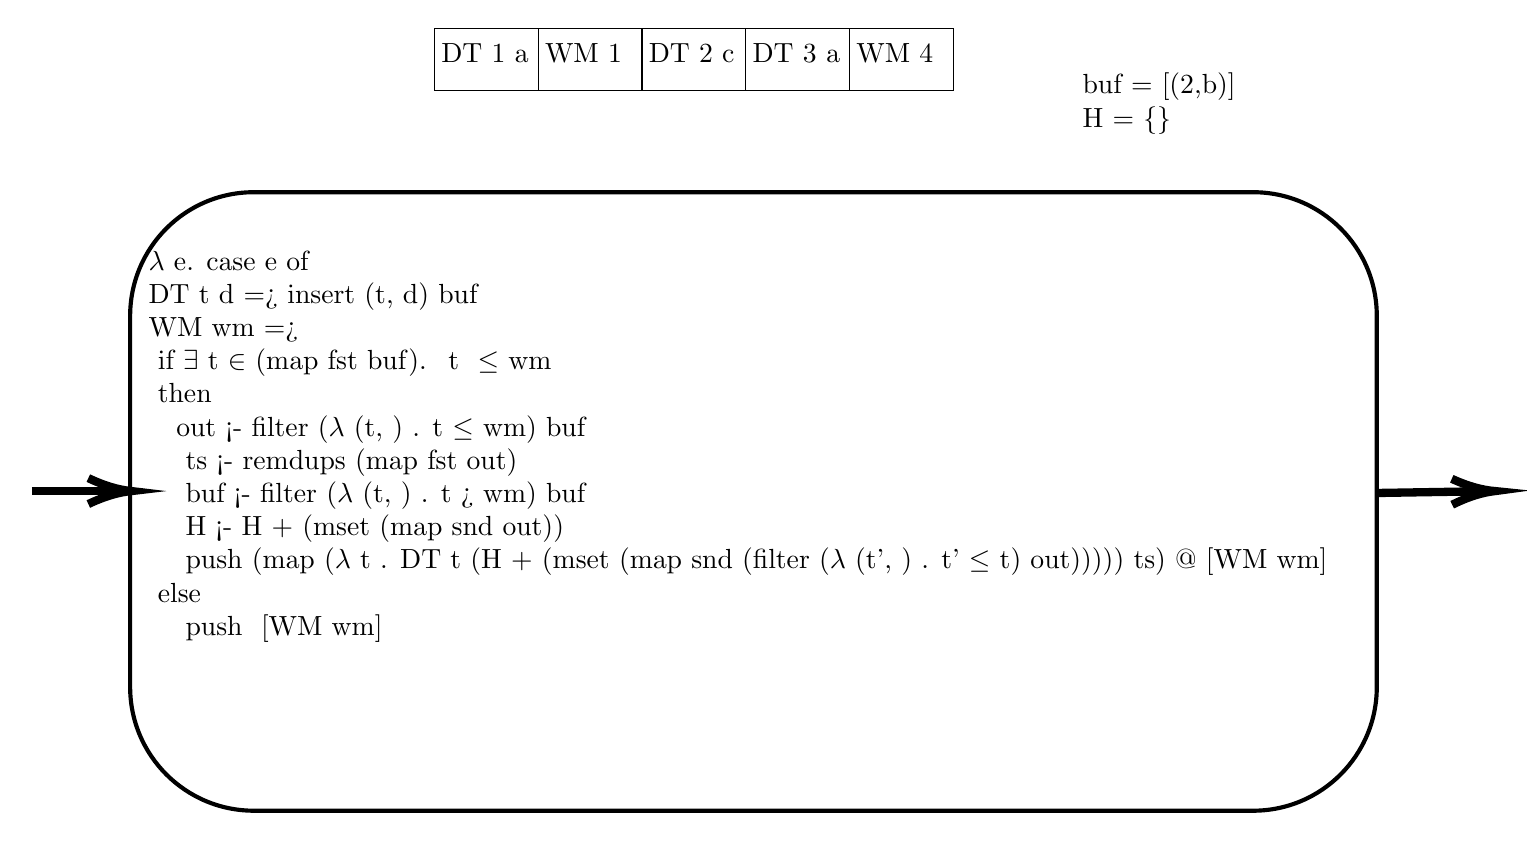
\begin{tikzpicture}[x=0.75pt,y=0.75pt,yscale=-1,xscale=1]
%uncomment if require: \path (0,489); %set diagram left start at 0, and has height of 489

%Rounded Rect [id:dp2828185464138784]
\draw  [line width=1.5]  (47.37,174.6) .. controls (47.37,141.68) and (74.05,115) .. (106.97,115) -- (588.4,115) .. controls (621.32,115) and (648,141.68) .. (648,174.6) -- (648,353.4) .. controls (648,386.32) and (621.32,413) .. (588.4,413) -- (106.97,413) .. controls (74.05,413) and (47.37,386.32) .. (47.37,353.4) -- cycle ;
%Shape: Rectangle [id:dp16185128837259355]
\draw   (194,36) -- (244,36) -- (244,66) -- (194,66) -- cycle ;
%Shape: Rectangle [id:dp07527633485084895]
\draw   (244,36) -- (294,36) -- (294,66) -- (244,66) -- cycle ;
%Shape: Rectangle [id:dp6518760155585928]
\draw   (294,36) -- (344,36) -- (344,66) -- (294,66) -- cycle ;
%Shape: Rectangle [id:dp8004967249958459]
\draw   (344,36) -- (394,36) -- (394,66) -- (344,66) -- cycle ;
%Shape: Rectangle [id:dp6426296003908789]
\draw   (394,36) -- (444,36) -- (444,66) -- (394,66) -- cycle ;
%Straight Lines [id:da3914639201104144]
\draw [line width=3]    (0,259) -- (43,259) ;
\draw [shift={(48,259)}, rotate = 180] [color={rgb, 255:red, 0; green, 0; blue, 0 }  ][line width=3]    (20.77,-6.25) .. controls (13.2,-2.65) and (6.28,-0.57) .. (0,0) .. controls (6.28,0.57) and (13.2,2.66) .. (20.77,6.25)   ;
%Straight Lines [id:da5752451790936068]
\draw [line width=3]    (648,259.92) -- (700,259.08) ;
\draw [shift={(705,259)}, rotate = 179.08] [color={rgb, 255:red, 0; green, 0; blue, 0 }  ][line width=3]    (20.77,-6.25) .. controls (13.2,-2.65) and (6.28,-0.57) .. (0,0) .. controls (6.28,0.57) and (13.2,2.66) .. (20.77,6.25)   ;

% Text Node
\draw (196,42) node [anchor=north west][inner sep=0.75pt]   [align=left] {DT 1 a};
% Text Node
\draw (246,42) node [anchor=north west][inner sep=0.75pt]   [align=left] {WM 1 };
% Text Node
\draw (296,42) node [anchor=north west][inner sep=0.75pt]   [align=left] {DT 2 c};
% Text Node
\draw (346,42) node [anchor=north west][inner sep=0.75pt]   [align=left] {DT 3 a};
% Text Node
\draw (396,42) node [anchor=north west][inner sep=0.75pt]   [align=left] {WM 4};
% Text Node
\draw (55,142) node [anchor=north west][inner sep=0.75pt]   [align=left] {$\lambda$ e. case e of\\DT t d => insert (t, d) buf\\WM wm =>\\ \ if $\exists$ t $\in$ (map fst buf). \ t \ $\le$ wm\\ \ then\\ \ \ \ out <- filter ($\lambda$ (t, \_) . t $\le$ wm) buf\\ \ \ \ \ ts <- remdups (map fst out)\\ \ \ \ \ buf <- filter ($\lambda$ (t, \_) . t > wm) buf\\ \ \ \ \ H <- H + (mset (map snd out))\\ \ \ \ \ push (map ($\lambda$ t . DT t (H + (mset (map snd (filter ($\lambda$ (t', \_) . t' $\le$ t) out))))) ts) @ [WM wm]\\ \ else\\ \ \ \ \ push \ [WM wm]};
% Text Node
\draw (505,56.33) node [anchor=north west][inner sep=0.75pt]   [align=left] {buf = [(2,b)]\\H = \{\}};


\end{tikzpicture}

  }
\end{frame}

\begin{frame}[fragile, noframenumbering]
  \frametitle{Example Time-Aware Stream Processing}
  \resizebox{0.9\textwidth}{0.8\textheight}{%


\tikzset{every picture/.style={line width=0.75pt}} %set default line width to 0.75pt

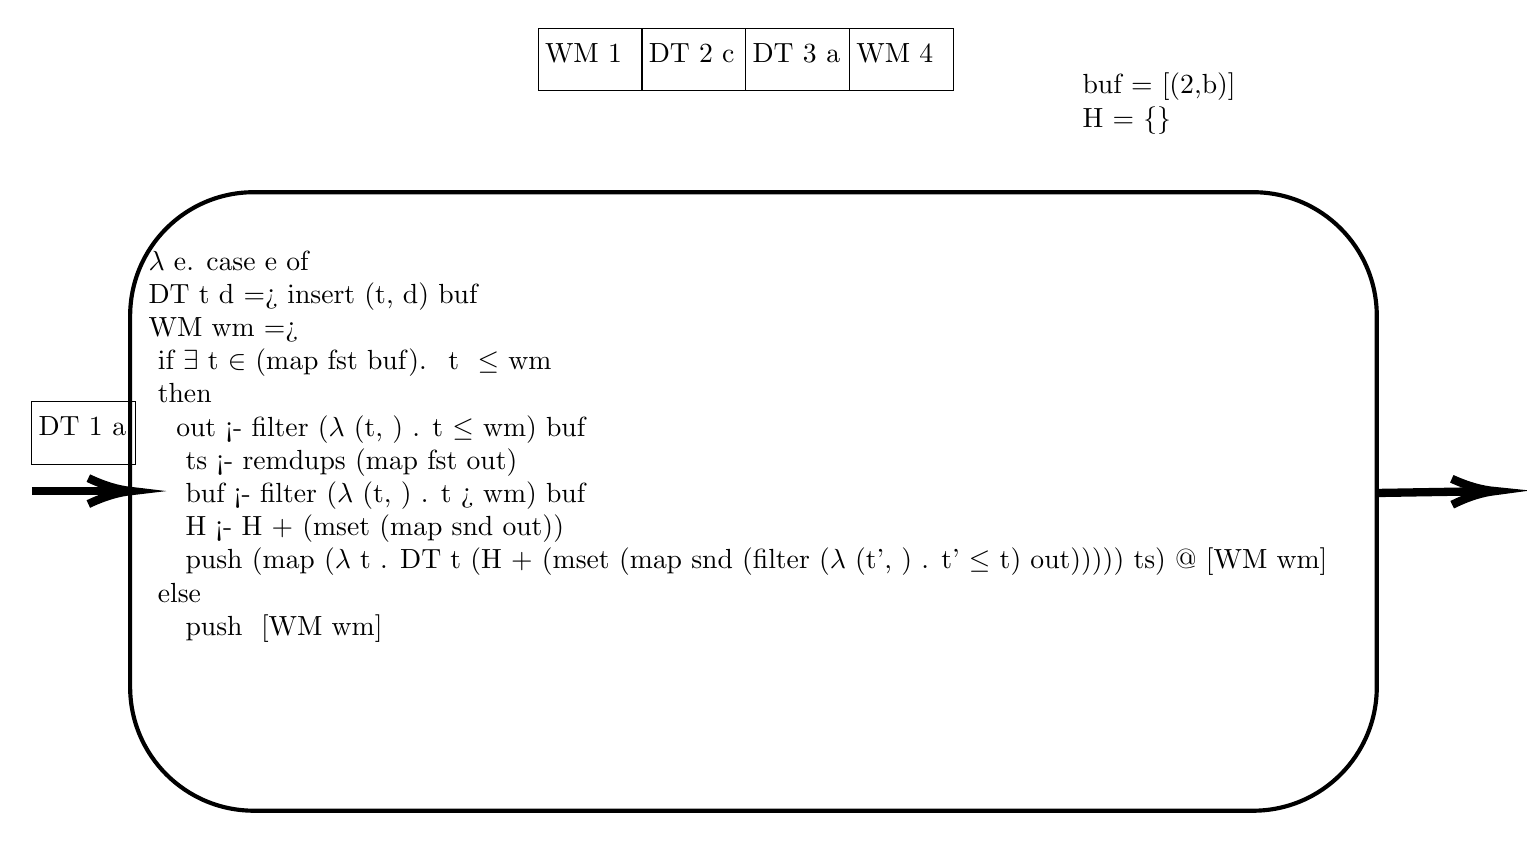
\begin{tikzpicture}[x=0.75pt,y=0.75pt,yscale=-1,xscale=1]
%uncomment if require: \path (0,489); %set diagram left start at 0, and has height of 489

%Rounded Rect [id:dp2828185464138784]
\draw  [line width=1.5]  (47.37,174.6) .. controls (47.37,141.68) and (74.05,115) .. (106.97,115) -- (588.4,115) .. controls (621.32,115) and (648,141.68) .. (648,174.6) -- (648,353.4) .. controls (648,386.32) and (621.32,413) .. (588.4,413) -- (106.97,413) .. controls (74.05,413) and (47.37,386.32) .. (47.37,353.4) -- cycle ;
%Shape: Rectangle [id:dp16185128837259355]
\draw   (0,216) -- (50,216) -- (50,246) -- (0,246) -- cycle ;
%Shape: Rectangle [id:dp07527633485084895]
\draw   (244,36) -- (294,36) -- (294,66) -- (244,66) -- cycle ;
%Shape: Rectangle [id:dp6518760155585928]
\draw   (294,36) -- (344,36) -- (344,66) -- (294,66) -- cycle ;
%Shape: Rectangle [id:dp8004967249958459]
\draw   (344,36) -- (394,36) -- (394,66) -- (344,66) -- cycle ;
%Shape: Rectangle [id:dp6426296003908789]
\draw   (394,36) -- (444,36) -- (444,66) -- (394,66) -- cycle ;
%Straight Lines [id:da3914639201104144]
\draw [line width=3]    (0,259) -- (43,259) ;
\draw [shift={(48,259)}, rotate = 180] [color={rgb, 255:red, 0; green, 0; blue, 0 }  ][line width=3]    (20.77,-6.25) .. controls (13.2,-2.65) and (6.28,-0.57) .. (0,0) .. controls (6.28,0.57) and (13.2,2.66) .. (20.77,6.25)   ;
%Straight Lines [id:da5752451790936068]
\draw [line width=3]    (648,259.92) -- (700,259.08) ;
\draw [shift={(705,259)}, rotate = 179.08] [color={rgb, 255:red, 0; green, 0; blue, 0 }  ][line width=3]    (20.77,-6.25) .. controls (13.2,-2.65) and (6.28,-0.57) .. (0,0) .. controls (6.28,0.57) and (13.2,2.66) .. (20.77,6.25)   ;

% Text Node
\draw (2,222) node [anchor=north west][inner sep=0.75pt]   [align=left] {DT 1 a};
% Text Node
\draw (246,42) node [anchor=north west][inner sep=0.75pt]   [align=left] {WM 1 };
% Text Node
\draw (296,42) node [anchor=north west][inner sep=0.75pt]   [align=left] {DT 2 c};
% Text Node
\draw (346,42) node [anchor=north west][inner sep=0.75pt]   [align=left] {DT 3 a};
% Text Node
\draw (396,42) node [anchor=north west][inner sep=0.75pt]   [align=left] {WM 4};
% Text Node
\draw (55,142) node [anchor=north west][inner sep=0.75pt]   [align=left] {$\lambda$ e. case e of\\DT t d => insert (t, d) buf\\WM wm =>\\ \ if $\exists$ t $\in$ (map fst buf). \ t \ $\le$ wm\\ \ then\\ \ \ \ out <- filter ($\lambda$ (t, \_) . t $\le$ wm) buf\\ \ \ \ \ ts <- remdups (map fst out)\\ \ \ \ \ buf <- filter ($\lambda$ (t, \_) . t > wm) buf\\ \ \ \ \ H <- H + (mset (map snd out))\\ \ \ \ \ push (map ($\lambda$ t . DT t (H + (mset (map snd (filter ($\lambda$ (t', \_) . t' $\le$ t) out))))) ts) @ [WM wm]\\ \ else\\ \ \ \ \ push \ [WM wm]};
% Text Node
\draw (505,56.33) node [anchor=north west][inner sep=0.75pt]   [align=left] {buf = [(2,b)]\\H = \{\}};


\end{tikzpicture}

  }
\end{frame}

\begin{frame}[fragile, noframenumbering]
  \frametitle{Example Time-Aware Stream Processing}
  \resizebox{0.9\textwidth}{0.8\textheight}{%


\tikzset{every picture/.style={line width=0.75pt}} %set default line width to 0.75pt

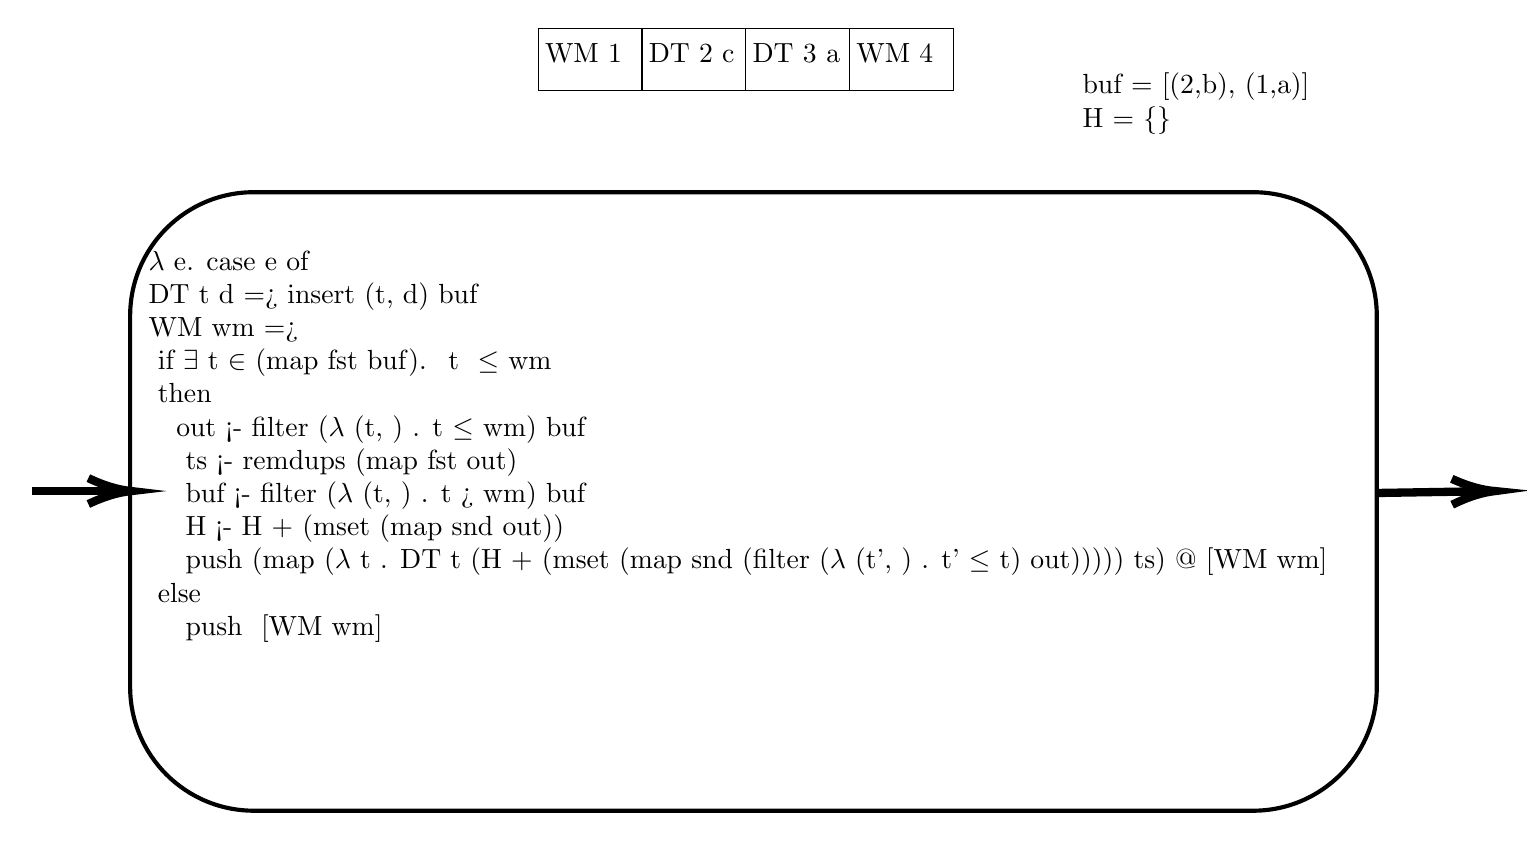
\begin{tikzpicture}[x=0.75pt,y=0.75pt,yscale=-1,xscale=1]
%uncomment if require: \path (0,489); %set diagram left start at 0, and has height of 489

%Rounded Rect [id:dp2828185464138784]
\draw  [line width=1.5]  (47.37,174.6) .. controls (47.37,141.68) and (74.05,115) .. (106.97,115) -- (588.4,115) .. controls (621.32,115) and (648,141.68) .. (648,174.6) -- (648,353.4) .. controls (648,386.32) and (621.32,413) .. (588.4,413) -- (106.97,413) .. controls (74.05,413) and (47.37,386.32) .. (47.37,353.4) -- cycle ;
%Shape: Rectangle [id:dp07527633485084895]
\draw   (244,36) -- (294,36) -- (294,66) -- (244,66) -- cycle ;
%Shape: Rectangle [id:dp6518760155585928]
\draw   (294,36) -- (344,36) -- (344,66) -- (294,66) -- cycle ;
%Shape: Rectangle [id:dp8004967249958459]
\draw   (344,36) -- (394,36) -- (394,66) -- (344,66) -- cycle ;
%Shape: Rectangle [id:dp6426296003908789]
\draw   (394,36) -- (444,36) -- (444,66) -- (394,66) -- cycle ;
%Straight Lines [id:da3914639201104144]
\draw [line width=3]    (0,259) -- (43,259) ;
\draw [shift={(48,259)}, rotate = 180] [color={rgb, 255:red, 0; green, 0; blue, 0 }  ][line width=3]    (20.77,-6.25) .. controls (13.2,-2.65) and (6.28,-0.57) .. (0,0) .. controls (6.28,0.57) and (13.2,2.66) .. (20.77,6.25)   ;
%Straight Lines [id:da5752451790936068]
\draw [line width=3]    (648,259.92) -- (700,259.08) ;
\draw [shift={(705,259)}, rotate = 179.08] [color={rgb, 255:red, 0; green, 0; blue, 0 }  ][line width=3]    (20.77,-6.25) .. controls (13.2,-2.65) and (6.28,-0.57) .. (0,0) .. controls (6.28,0.57) and (13.2,2.66) .. (20.77,6.25)   ;

% Text Node
\draw (246,42) node [anchor=north west][inner sep=0.75pt]   [align=left] {WM 1 };
% Text Node
\draw (296,42) node [anchor=north west][inner sep=0.75pt]   [align=left] {DT 2 c};
% Text Node
\draw (346,42) node [anchor=north west][inner sep=0.75pt]   [align=left] {DT 3 a};
% Text Node
\draw (396,42) node [anchor=north west][inner sep=0.75pt]   [align=left] {WM 4};
% Text Node
\draw (55,142) node [anchor=north west][inner sep=0.75pt]   [align=left] {$\lambda$ e. case e of\\DT t d => insert (t, d) buf\\WM wm =>\\ \ if $\exists$ t $\in$ (map fst buf). \ t \ $\le$ wm\\ \ then\\ \ \ \ out <- filter ($\lambda$ (t, \_) . t $\le$ wm) buf\\ \ \ \ \ ts <- remdups (map fst out)\\ \ \ \ \ buf <- filter ($\lambda$ (t, \_) . t > wm) buf\\ \ \ \ \ H <- H + (mset (map snd out))\\ \ \ \ \ push (map ($\lambda$ t . DT t (H + (mset (map snd (filter ($\lambda$ (t', \_) . t' $\le$ t) out))))) ts) @ [WM wm]\\ \ else\\ \ \ \ \ push \ [WM wm]};
% Text Node
\draw (505,56.33) node [anchor=north west][inner sep=0.75pt]   [align=left] {buf = [(2,b), (1,a)]\\H = \{\}};


\end{tikzpicture}

  }
\end{frame}


\begin{frame}[fragile, noframenumbering]
  \frametitle{Example Time-Aware Stream Processing}
  \resizebox{0.9\textwidth}{0.8\textheight}{%


\tikzset{every picture/.style={line width=0.75pt}} %set default line width to 0.75pt

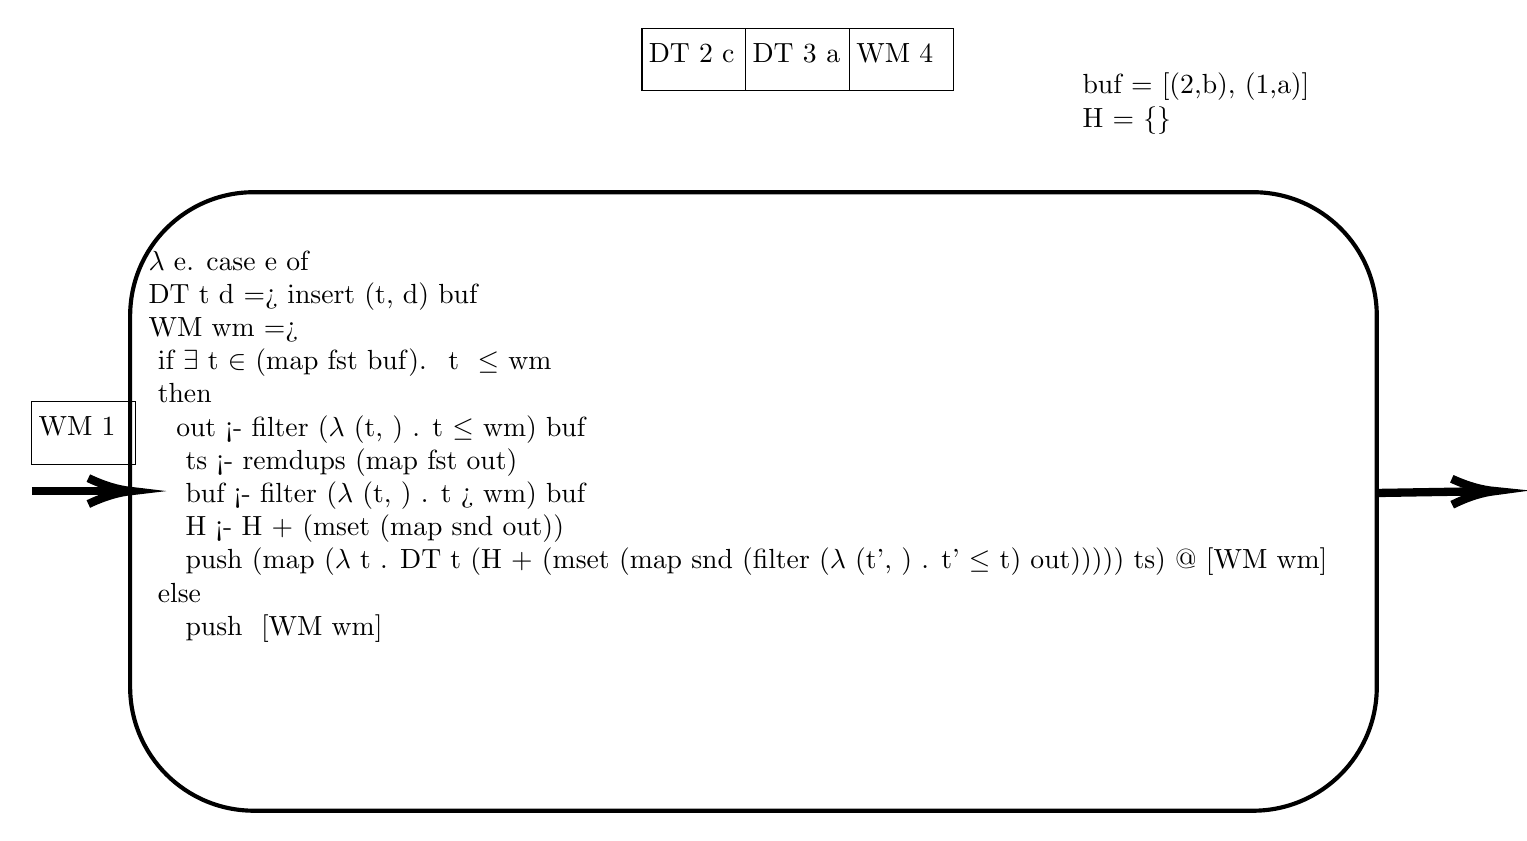
\begin{tikzpicture}[x=0.75pt,y=0.75pt,yscale=-1,xscale=1]
%uncomment if require: \path (0,489); %set diagram left start at 0, and has height of 489

%Rounded Rect [id:dp2828185464138784]
\draw  [line width=1.5]  (47.37,174.6) .. controls (47.37,141.68) and (74.05,115) .. (106.97,115) -- (588.4,115) .. controls (621.32,115) and (648,141.68) .. (648,174.6) -- (648,353.4) .. controls (648,386.32) and (621.32,413) .. (588.4,413) -- (106.97,413) .. controls (74.05,413) and (47.37,386.32) .. (47.37,353.4) -- cycle ;
%Shape: Rectangle [id:dp07527633485084895]
\draw   (0,216) -- (50,216) -- (50,246) -- (0,246) -- cycle ;
%Shape: Rectangle [id:dp6518760155585928]
\draw   (294,36) -- (344,36) -- (344,66) -- (294,66) -- cycle ;
%Shape: Rectangle [id:dp8004967249958459]
\draw   (344,36) -- (394,36) -- (394,66) -- (344,66) -- cycle ;
%Shape: Rectangle [id:dp6426296003908789]
\draw   (394,36) -- (444,36) -- (444,66) -- (394,66) -- cycle ;
%Straight Lines [id:da3914639201104144]
\draw [line width=3]    (0,259) -- (43,259) ;
\draw [shift={(48,259)}, rotate = 180] [color={rgb, 255:red, 0; green, 0; blue, 0 }  ][line width=3]    (20.77,-6.25) .. controls (13.2,-2.65) and (6.28,-0.57) .. (0,0) .. controls (6.28,0.57) and (13.2,2.66) .. (20.77,6.25)   ;
%Straight Lines [id:da5752451790936068]
\draw [line width=3]    (648,259.92) -- (700,259.08) ;
\draw [shift={(705,259)}, rotate = 179.08] [color={rgb, 255:red, 0; green, 0; blue, 0 }  ][line width=3]    (20.77,-6.25) .. controls (13.2,-2.65) and (6.28,-0.57) .. (0,0) .. controls (6.28,0.57) and (13.2,2.66) .. (20.77,6.25)   ;

% Text Node
\draw (2,222) node [anchor=north west][inner sep=0.75pt]   [align=left] {WM 1 };
% Text Node
\draw (296,42) node [anchor=north west][inner sep=0.75pt]   [align=left] {DT 2 c};
% Text Node
\draw (346,42) node [anchor=north west][inner sep=0.75pt]   [align=left] {DT 3 a};
% Text Node
\draw (396,42) node [anchor=north west][inner sep=0.75pt]   [align=left] {WM 4};
% Text Node
\draw (55,142) node [anchor=north west][inner sep=0.75pt]   [align=left] {$\lambda$ e. case e of\\DT t d => insert (t, d) buf\\WM wm =>\\ \ if $\exists$ t $\in$ (map fst buf). \ t \ $\le$ wm\\ \ then\\ \ \ \ out <- filter ($\lambda$ (t, \_) . t $\le$ wm) buf\\ \ \ \ \ ts <- remdups (map fst out)\\ \ \ \ \ buf <- filter ($\lambda$ (t, \_) . t > wm) buf\\ \ \ \ \ H <- H + (mset (map snd out))\\ \ \ \ \ push (map ($\lambda$ t . DT t (H + (mset (map snd (filter ($\lambda$ (t', \_) . t' $\le$ t) out))))) ts) @ [WM wm]\\ \ else\\ \ \ \ \ push \ [WM wm]};
% Text Node
\draw (505,56.33) node [anchor=north west][inner sep=0.75pt]   [align=left] {buf = [(2,b), (1,a)]\\H = \{\}};


\end{tikzpicture}

  }
\end{frame}

\begin{frame}[fragile, noframenumbering]
  \frametitle{Example Time-Aware Stream Processing}
  \resizebox{0.9\textwidth}{0.8\textheight}{%


\tikzset{every picture/.style={line width=0.75pt}} %set default line width to 0.75pt

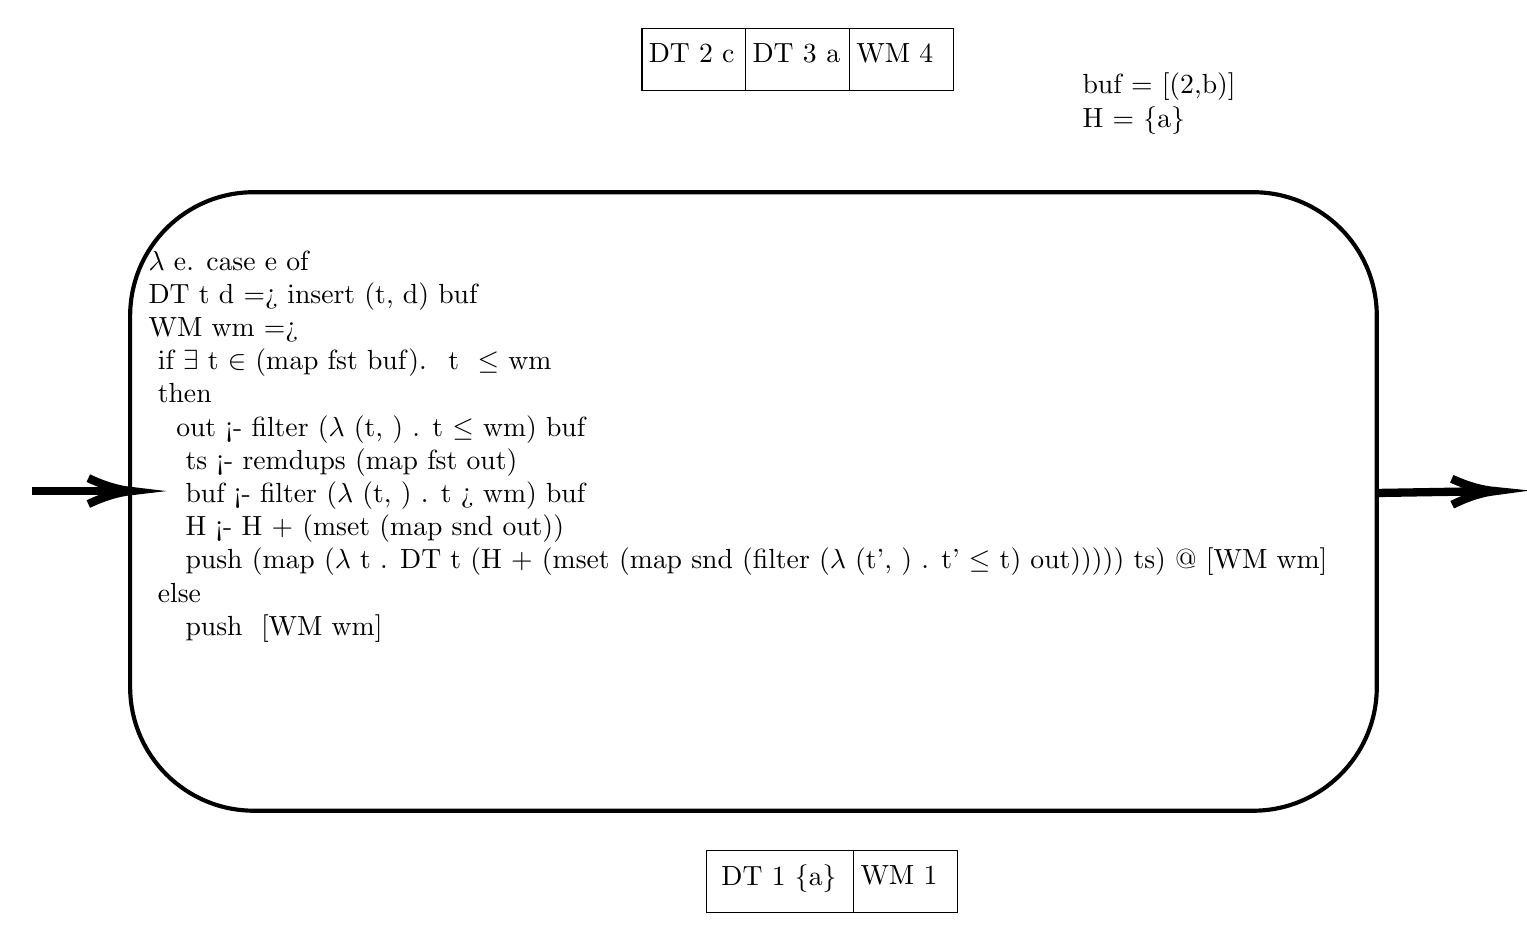
\begin{tikzpicture}[x=0.75pt,y=0.75pt,yscale=-1,xscale=1]
%uncomment if require: \path (0,489); %set diagram left start at 0, and has height of 489

%Rounded Rect [id:dp2828185464138784]
\draw  [line width=1.5]  (47.37,174.6) .. controls (47.37,141.68) and (74.05,115) .. (106.97,115) -- (588.4,115) .. controls (621.32,115) and (648,141.68) .. (648,174.6) -- (648,353.4) .. controls (648,386.32) and (621.32,413) .. (588.4,413) -- (106.97,413) .. controls (74.05,413) and (47.37,386.32) .. (47.37,353.4) -- cycle ;
%Shape: Rectangle [id:dp07527633485084895]
\draw   (396,432) -- (446,432) -- (446,462) -- (396,462) -- cycle ;
%Shape: Rectangle [id:dp6518760155585928]
\draw   (294,36) -- (344,36) -- (344,66) -- (294,66) -- cycle ;
%Shape: Rectangle [id:dp8004967249958459]
\draw   (344,36) -- (394,36) -- (394,66) -- (344,66) -- cycle ;
%Shape: Rectangle [id:dp6426296003908789]
\draw   (394,36) -- (444,36) -- (444,66) -- (394,66) -- cycle ;
%Straight Lines [id:da3914639201104144]
\draw [line width=3]    (0,259) -- (43,259) ;
\draw [shift={(48,259)}, rotate = 180] [color={rgb, 255:red, 0; green, 0; blue, 0 }  ][line width=3]    (20.77,-6.25) .. controls (13.2,-2.65) and (6.28,-0.57) .. (0,0) .. controls (6.28,0.57) and (13.2,2.66) .. (20.77,6.25)   ;
%Straight Lines [id:da5752451790936068]
\draw [line width=3]    (648,259.92) -- (700,259.08) ;
\draw [shift={(705,259)}, rotate = 179.08] [color={rgb, 255:red, 0; green, 0; blue, 0 }  ][line width=3]    (20.77,-6.25) .. controls (13.2,-2.65) and (6.28,-0.57) .. (0,0) .. controls (6.28,0.57) and (13.2,2.66) .. (20.77,6.25)   ;
%Shape: Rectangle [id:dp9360080992935229]
\draw   (325,432) -- (396,432) -- (396,462) -- (325,462) -- cycle ;

% Text Node
\draw (398,438) node [anchor=north west][inner sep=0.75pt]   [align=left] {WM 1 };
% Text Node
\draw (296,42) node [anchor=north west][inner sep=0.75pt]   [align=left] {DT 2 c};
% Text Node
\draw (346,42) node [anchor=north west][inner sep=0.75pt]   [align=left] {DT 3 a};
% Text Node
\draw (396,42) node [anchor=north west][inner sep=0.75pt]   [align=left] {WM 4};
% Text Node
\draw (55,142) node [anchor=north west][inner sep=0.75pt]   [align=left] {$\lambda$ e. case e of\\DT t d => insert (t, d) buf\\WM wm =>\\ \ if $\exists$ t $\in$ (map fst buf). \ t \ $\le$ wm\\ \ then\\ \ \ \ out <- filter ($\lambda$ (t, \_) . t $\le$ wm) buf\\ \ \ \ \ ts <- remdups (map fst out)\\ \ \ \ \ buf <- filter ($\lambda$ (t, \_) . t > wm) buf\\ \ \ \ \ H <- H + (mset (map snd out))\\ \ \ \ \ push (map ($\lambda$ t . DT t (H + (mset (map snd (filter ($\lambda$ (t', \_) . t' $\le$ t) out))))) ts) @ [WM wm]\\ \ else\\ \ \ \ \ push \ [WM wm]};
% Text Node
\draw (505,56.33) node [anchor=north west][inner sep=0.75pt]   [align=left] {buf = [(2,b)]\\H = \{a\}};
% Text Node
\draw (331,438) node [anchor=north west][inner sep=0.75pt]   [align=left] {DT 1 \{a\}};


\end{tikzpicture}

  }
\end{frame}

\begin{frame}[fragile, noframenumbering]
  \frametitle{Example Time-Aware Stream Processing}
  \resizebox{0.9\textwidth}{0.8\textheight}{%


\tikzset{every picture/.style={line width=0.75pt}} %set default line width to 0.75pt

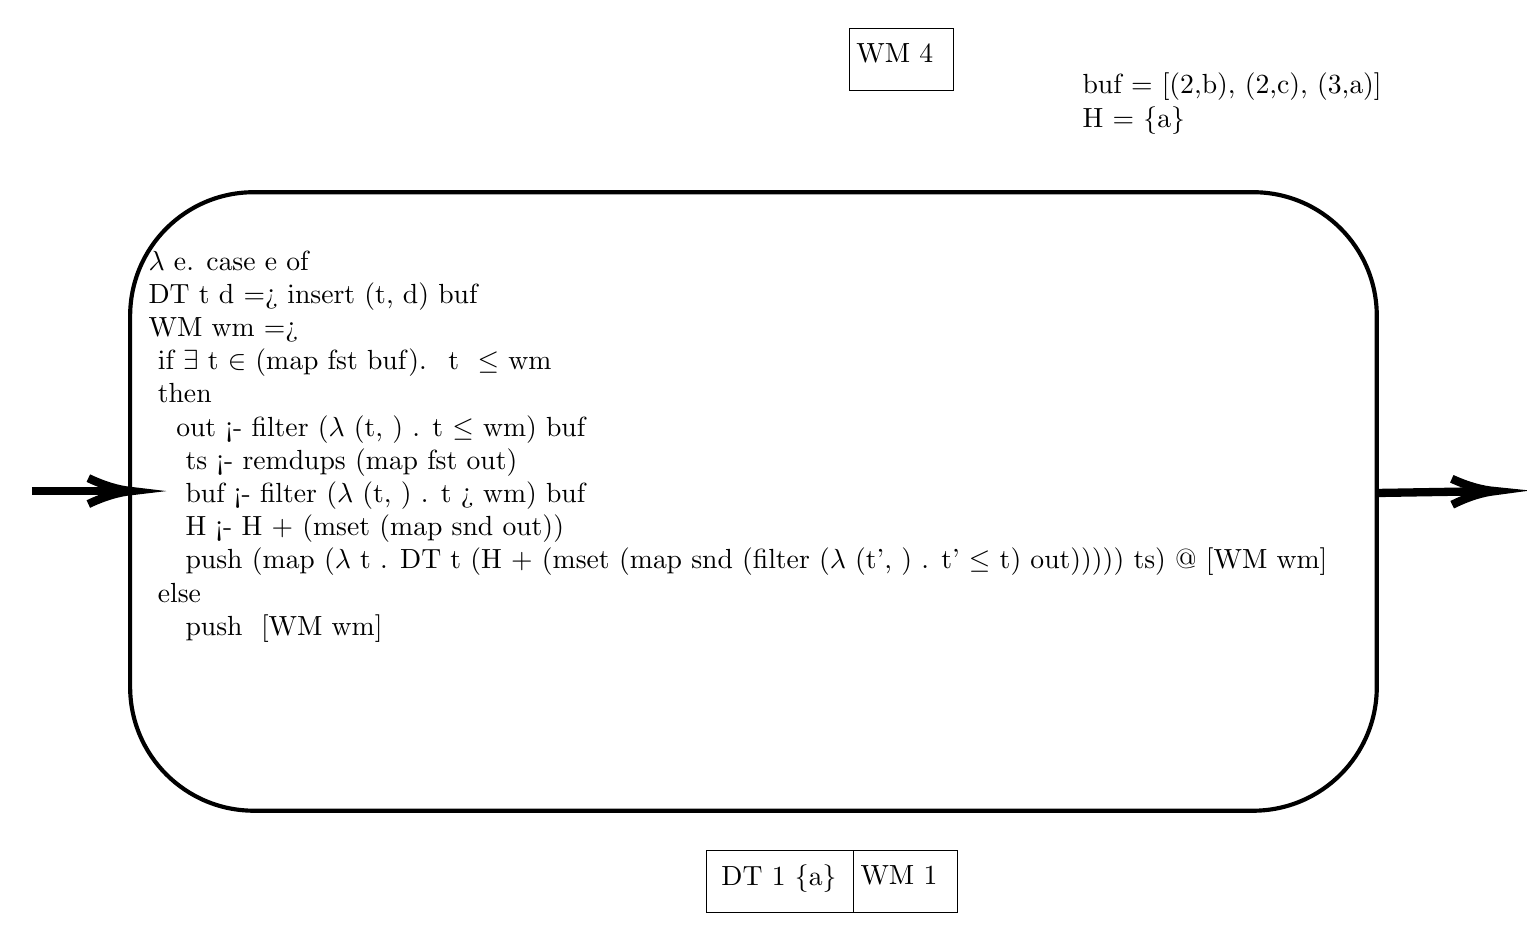
\begin{tikzpicture}[x=0.75pt,y=0.75pt,yscale=-1,xscale=1]
%uncomment if require: \path (0,489); %set diagram left start at 0, and has height of 489

%Rounded Rect [id:dp2828185464138784]
\draw  [line width=1.5]  (47.37,174.6) .. controls (47.37,141.68) and (74.05,115) .. (106.97,115) -- (588.4,115) .. controls (621.32,115) and (648,141.68) .. (648,174.6) -- (648,353.4) .. controls (648,386.32) and (621.32,413) .. (588.4,413) -- (106.97,413) .. controls (74.05,413) and (47.37,386.32) .. (47.37,353.4) -- cycle ;
%Shape: Rectangle [id:dp07527633485084895]
\draw   (396,432) -- (446,432) -- (446,462) -- (396,462) -- cycle ;
%Shape: Rectangle [id:dp6426296003908789]
\draw   (394,36) -- (444,36) -- (444,66) -- (394,66) -- cycle ;
%Straight Lines [id:da3914639201104144]
\draw [line width=3]    (0,259) -- (43,259) ;
\draw [shift={(48,259)}, rotate = 180] [color={rgb, 255:red, 0; green, 0; blue, 0 }  ][line width=3]    (20.77,-6.25) .. controls (13.2,-2.65) and (6.28,-0.57) .. (0,0) .. controls (6.28,0.57) and (13.2,2.66) .. (20.77,6.25)   ;
%Straight Lines [id:da5752451790936068]
\draw [line width=3]    (648,259.92) -- (700,259.08) ;
\draw [shift={(705,259)}, rotate = 179.08] [color={rgb, 255:red, 0; green, 0; blue, 0 }  ][line width=3]    (20.77,-6.25) .. controls (13.2,-2.65) and (6.28,-0.57) .. (0,0) .. controls (6.28,0.57) and (13.2,2.66) .. (20.77,6.25)   ;
%Shape: Rectangle [id:dp9360080992935229]
\draw   (325,432) -- (396,432) -- (396,462) -- (325,462) -- cycle ;

% Text Node
\draw (398,438) node [anchor=north west][inner sep=0.75pt]   [align=left] {WM 1 };
% Text Node
\draw (396,42) node [anchor=north west][inner sep=0.75pt]   [align=left] {WM 4};
% Text Node
\draw (55,142) node [anchor=north west][inner sep=0.75pt]   [align=left] {$\lambda$ e. case e of\\DT t d => insert (t, d) buf\\WM wm =>\\ \ if $\exists$ t $\in$ (map fst buf). \ t \ $\le$ wm\\ \ then\\ \ \ \ out <- filter ($\lambda$ (t, \_) . t $\le$ wm) buf\\ \ \ \ \ ts <- remdups (map fst out)\\ \ \ \ \ buf <- filter ($\lambda$ (t, \_) . t > wm) buf\\ \ \ \ \ H <- H + (mset (map snd out))\\ \ \ \ \ push (map ($\lambda$ t . DT t (H + (mset (map snd (filter ($\lambda$ (t', \_) . t' $\le$ t) out))))) ts) @ [WM wm]\\ \ else\\ \ \ \ \ push \ [WM wm]};
% Text Node
\draw (505,56.33) node [anchor=north west][inner sep=0.75pt]   [align=left] {buf = [(2,b), (2,c), (3,a)]\\H = \{a\}};
% Text Node
\draw (331,438) node [anchor=north west][inner sep=0.75pt]   [align=left] {DT 1 \{a\}};


\end{tikzpicture}

  }
\end{frame}

\begin{frame}[fragile, noframenumbering]
  \frametitle{Example Time-Aware Stream Processing}
  \resizebox{0.9\textwidth}{0.8\textheight}{%


\tikzset{every picture/.style={line width=0.75pt}} %set default line width to 0.75pt

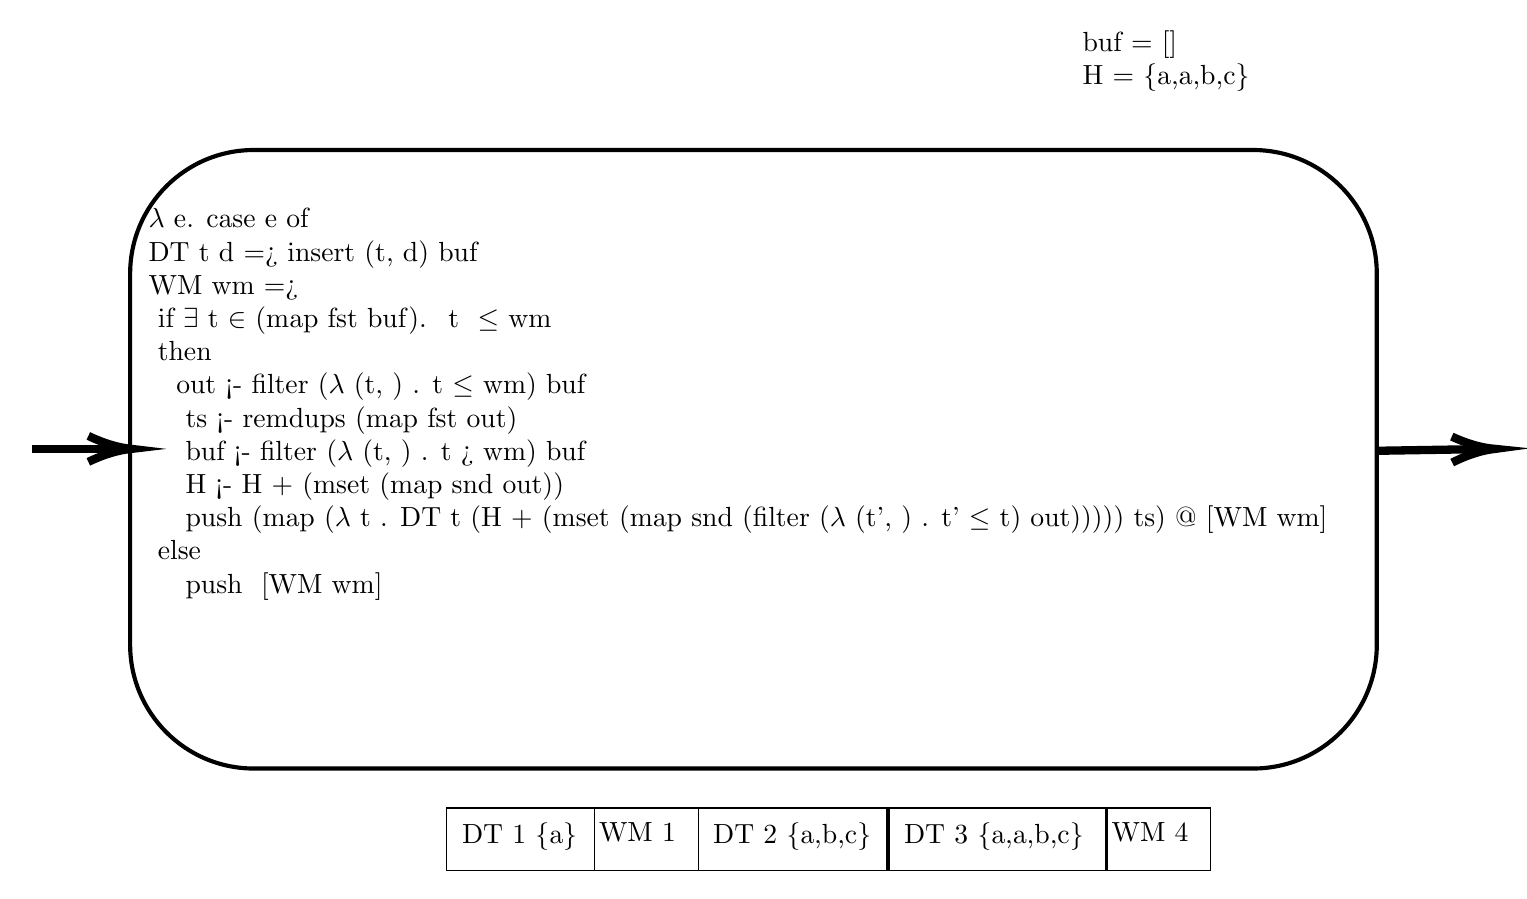
\begin{tikzpicture}[x=0.75pt,y=0.75pt,yscale=-1,xscale=1]
%uncomment if require: \path (0,489); %set diagram left start at 0, and has height of 489

%Rounded Rect [id:dp2828185464138784]
\draw  [line width=1.5]  (47.37,174.6) .. controls (47.37,141.68) and (74.05,115) .. (106.97,115) -- (588.4,115) .. controls (621.32,115) and (648,141.68) .. (648,174.6) -- (648,353.4) .. controls (648,386.32) and (621.32,413) .. (588.4,413) -- (106.97,413) .. controls (74.05,413) and (47.37,386.32) .. (47.37,353.4) -- cycle ;
%Shape: Rectangle [id:dp07527633485084895]
\draw   (271,432) -- (321,432) -- (321,462) -- (271,462) -- cycle ;
%Straight Lines [id:da3914639201104144]
\draw [line width=3]    (0,259) -- (43,259) ;
\draw [shift={(48,259)}, rotate = 180] [color={rgb, 255:red, 0; green, 0; blue, 0 }  ][line width=3]    (20.77,-6.25) .. controls (13.2,-2.65) and (6.28,-0.57) .. (0,0) .. controls (6.28,0.57) and (13.2,2.66) .. (20.77,6.25)   ;
%Straight Lines [id:da5752451790936068]
\draw [line width=3]    (648,259.92) -- (700,259.08) ;
\draw [shift={(705,259)}, rotate = 179.08] [color={rgb, 255:red, 0; green, 0; blue, 0 }  ][line width=3]    (20.77,-6.25) .. controls (13.2,-2.65) and (6.28,-0.57) .. (0,0) .. controls (6.28,0.57) and (13.2,2.66) .. (20.77,6.25)   ;
%Shape: Rectangle [id:dp9360080992935229]
\draw   (200,432) -- (271,432) -- (271,462) -- (200,462) -- cycle ;
%Shape: Rectangle [id:dp025487318872198017]
\draw   (518,432) -- (568,432) -- (568,462) -- (518,462) -- cycle ;
%Shape: Rectangle [id:dp6091069098377138]
\draw   (321,432) -- (412,432) -- (412,462) -- (321,462) -- cycle ;
%Shape: Rectangle [id:dp12580135752131838]
\draw   (413,432) -- (517.5,432) -- (517.5,462) -- (413,462) -- cycle ;

% Text Node
\draw (272,438) node [anchor=north west][inner sep=0.75pt]   [align=left] {WM 1 };
% Text Node
\draw (55,142) node [anchor=north west][inner sep=0.75pt]   [align=left] {$\lambda$ e. case e of\\DT t d => insert (t, d) buf\\WM wm =>\\ \ if $\exists$ t $\in$ (map fst buf). \ t \ $\le$ wm\\ \ then\\ \ \ \ out <- filter ($\lambda$ (t, \_) . t $\le$ wm) buf\\ \ \ \ \ ts <- remdups (map fst out)\\ \ \ \ \ buf <- filter ($\lambda$ (t, \_) . t > wm) buf\\ \ \ \ \ H <- H + (mset (map snd out))\\ \ \ \ \ push (map ($\lambda$ t . DT t (H + (mset (map snd (filter ($\lambda$ (t', \_) . t' $\le$ t) out))))) ts) @ [WM wm]\\ \ else\\ \ \ \ \ push \ [WM wm]};
% Text Node
\draw (505,56.33) node [anchor=north west][inner sep=0.75pt]   [align=left] {buf = []\\H = \{a,a,b,c\}};
% Text Node
\draw (206,438) node [anchor=north west][inner sep=0.75pt]   [align=left] {DT 1 \{a\}};
% Text Node
\draw (519,438) node [anchor=north west][inner sep=0.75pt]   [align=left] {WM 4 };
% Text Node
\draw (327,438) node [anchor=north west][inner sep=0.75pt]   [align=left] {DT 2 \{a,b,c\}};
% Text Node
\draw (419,438) node [anchor=north west][inner sep=0.75pt]   [align=left] {DT 3 \{a,a,b,c\}};


\end{tikzpicture}

  }
\end{frame}

\section{Preliminaries}
\begin{frame}[fragile]
  \frametitle{Isabelle/HOL}
  \begin{itemize}
    \item Classical higher-order logic (HOL): Simple Typed Lambda Calculus + (Hilbert) axiom of choice + axiom of infinity + rank-1 polymorphism
          \pause
    \item Isabelle: A generic proof assistant
          \begin{overlayarea}{\textwidth}{.45\textheight}
            \centering
            \begin{figure}
              \centering
              \only<2>{
\includegraphics[scale=0.15]{isabelle}}
            \end{figure}
          \end{overlayarea}
    \item Isabelle/HOL: Isabelle's flavor of HOL
  \end{itemize}
\end{frame}

\begin{frame}[fragile]
  \frametitle{Isabelle/HOL: (Co)datatypes}
  \begin{itemize}
    \item Datatypes and Codatatypes
\vspace*{-1ex}
          \begin{tcblisting}{hbox,listing only,listing options={language=isabelle,aboveskip=0pt,belowskip=0pt},size=fbox,boxrule=0pt,frame hidden,arc=0pt,colback=yellow!10!white}
codatatype (lset: 'a) llist = lnull: LNil | LCons (lhd: 'a) (ltl: "'a llist")
  for map: lmap where "ltl LNil = LNil"
          \end{tcblisting}
\vspace*{-1ex}
    \item Examples:
          \begin{itemize}
            \item \is{LNil}
            \item \is{LCons 1 (LCons 2 (LCons 3 LNil))}
            \item \is{LCons 0 (LCons 0 (LCons 0 (...)))}
          \end{itemize}
\vspace*{-1ex}
    \item Proofs by induction
    \item Proofs by coinduction
  \end{itemize}
\end{frame}

\section{State of this work}

\begin{frame}[fragile]
  \frametitle{What have I formalized so far? (part 1)}
  \begin{itemize}
    \item Formalization stream processing (model)
          \begin{itemize}
            \item Using Isabelle/HOL: (co)datatypes, (co)recursion, and (co)induction
            \item Streams are lazy lists, and operators as a codatatype
            \item Semantics: a \is{produce :: 'i llist => ('i, 'o) op => 'o llist} function that runs an operator throughout a lazy lists
                  \begin{itemize}
                    \item Mix of recursion and corecursion: inductive and coinductive principles
                  \end{itemize}
            \item Sequential composition
                  \begin{itemize}
                    \item Correctness!
                  \end{itemize}
          \end{itemize}
  \end{itemize}
\end{frame}

\begin{frame}[fragile]
  \frametitle{What have I formalized so far?  (part 2)}
  \begin{itemize}
    \item Time-Aware computations
          \begin{itemize}
            \item Coinductive properties of streams: monotonicity and productivity
            \item Building blocks operators:
                  \begin{itemize}
                    \item Convenience operators: batching and incremental computations
                          \begin{itemize}
                            \item Incremental computing: only update results that are affected by the new input
                            \item With verified properties: Soundness, Completeness, preservation of monotonicity, and preservation of productivity
                          \end{itemize}
                  \end{itemize}
            \item Compositional reasoning
          \end{itemize}
    \item Case studies with the building blocks:
          \begin{itemize}
            \item Incremental histogram operator
            \item Relational join
          \end{itemize}
  \end{itemize}
\end{frame}

\section{Next Steps}

\begin{frame}[fragile]
  \frametitle{Efficient Stream Processing}
  \begin{itemize}
    \item It is executable! But slow!
          \begin{itemize}
            \item Code generator: functional languages (OCaml, Haskell, SML...)
            \item Functional data-structures (often not ideal)
          \end{itemize}
    \pause
    \item How do we make efficient and verified programs in Isabelle/HOL?
          \pause
          \item Isabelle-LLVM!
          \item Let's port this formalization to Isabelle-LLVM then!
    \item This is a non-terminating program
    \end{itemize}
\end{frame}

\section{Isabelle-LLVM}

\begin{frame}[fragile]
  \frametitle{Isabelle Refinement Framework and Isabelle-LLVM}
  \begin{itemize}
    \item Isabelle Refinement Framework
          \begin{itemize}
            \item Framework for step-wise refinement verification (refinement calculus): Specification $\rightarrow$ Abstract Algorithm $\rightarrow$ Less Abstract Algorithm $\rightarrow$ Executable Code
            \item Imperative HOL as backend (lowest layer in the refinement)
                  \begin{itemize}
                    \item Shallow Embedding of Monadic programs in HOL
                  \end{itemize}
            \item Separation Logic (heap memory reasoning)
          \end{itemize}
    \item Isabelle-LLVM is a new backend for the Isabelle Refinement Framework
          \begin{itemize}
            \item Generates LLVM code (efficient imperative code)
          \end{itemize}
          \pause
    \item Can we write and verify non-terminating programs in this framework?
          \pause
          \begin{itemize}
            \item Yes and No!
          \end{itemize}
  \end{itemize}
\end{frame}

\begin{frame}[fragile]
  \frametitle{Isabelle-LLVM's Recursion Model}
  \begin{itemize}
    \item Knaster–Tarski theorem
          \begin{itemize}
            \item Standard way to define the semantics of recursive definitions
                  \begin{itemize}
                    \item Isabelle/HOL: Partial Function Package
                  \end{itemize}
            \item Every monotonic function on Complete Chain Partial Order (CCPO) has a fixed point
            \item Induction principle
          \end{itemize}
    \item No need for well-foundness
  \end{itemize}
\end{frame}

\begin{frame}[fragile]
  \frametitle{What the Heck is a CCPO?}
  \begin{itemize}
    \item Chain: A set in which all elements are comparable
    \item Complete Chain Partial Order:
          \begin{enumerate}
            \item A partial order: \is{'a::order}
            \item A function that returns the suprimium (least upper bound) from a chain \is{'a::order set => 'a}
          \end{enumerate}
    \pause
    \item Isabelle-LLVM's monad:
          \vspace*{-1ex}
          \begin{tcblisting}{hbox,listing only,listing options={language=isabelle,aboveskip=0pt,belowskip=0pt},size=fbox,boxrule=0pt,frame hidden,arc=0pt,colback=yellow!10!white}
datatype 'a neM = SPEC (the_spec: "'a => bool") | FAIL
          \end{tcblisting}
          \vspace*{-1ex}
          \begin{itemize}
            \item Order: flat (every \is{SPEC} is greater than \is{FAIL}, \is{SPEC}s are only comparable when they are equal)
            \item Supremum from a chain: The \is{SPEC}, or the only \is{FAIL}
            \item Bottom: \is{FAIL}
                  \begin{itemize}
                    \item Non-termination
                  \end{itemize}
          \end{itemize}
  \end{itemize}
\end{frame}

\section{The First Steps}

\begin{frame}[fragile]
  \frametitle{Our CCPO Attempt}
  \begin{itemize}
    \item Let's look in Isabelle!
  \end{itemize}
\end{frame}

\section{The Other Steps}
\begin{frame}[fragile]
  \frametitle{More Changes to Isabelle-LLVM?}
  \begin{itemize}
    \item Separation Logic?
          \begin{itemize}
            \item Express properties about the trace of the program
          \end{itemize}
    \item Refinement Calculus?
    \item LLVM code generator?
  \end{itemize}
\end{frame}

\section{Questions, comments and suggestions}

\end{document}
